%definira klasu dokumenta 
\documentclass[12pt]{report} 

%prostor izmedu naredbi \documentclass i \begin{document} se zove uvod. U njemu se nalaze naredbe koje se odnose na cijeli dokument

%osnovni LaTex ne može riješiti sve probleme, pa se koriste različiti paketi koji olakšavaju izradu željenog dokumenta
\usepackage[croatian]{babel} 
\usepackage{amssymb}
\usepackage{amsmath}
\usepackage{txfonts}
\usepackage{mathdots}
\usepackage{titlesec}
\usepackage{array}
\usepackage{lastpage}
\usepackage{etoolbox}
\usepackage{tabularray}
\usepackage{color, colortbl}
\usepackage{adjustbox}
\usepackage{geometry}
\usepackage[classicReIm]{kpfonts}
\usepackage{hyperref}
\usepackage{fancyhdr}

\usepackage{float}
\usepackage{setspace}
\restylefloat{table}


\patchcmd{\chapter}{\thispagestyle{plain}}{\thispagestyle{fancy}}{}{} %redefiniranje stila stranice u paketu fancyhdr

%oblik naslova poglavlja
\titleformat{\chapter}{\normalfont\huge\bfseries}{\thechapter.}{20pt}{\Huge}
\titlespacing{\chapter}{0pt}{0pt}{40pt}


\linespread{1.3} %razmak između redaka

\geometry{a4paper, left=1in, top=1in,}  %oblik stranice

\hypersetup{ colorlinks, citecolor=black, filecolor=black, linkcolor=black,	urlcolor=black }   %izgled poveznice


%prored smanjen između redaka u nabrajanjima i popisima
\newenvironment{packed_enum}{
	\begin{enumerate}
		\setlength{\itemsep}{0pt}
		\setlength{\parskip}{0pt}
		\setlength{\parsep}{0pt}
	}{\end{enumerate}}

\newenvironment{packed_item}{
	\begin{itemize}
		\setlength{\itemsep}{0pt}
		\setlength{\parskip}{0pt}
		\setlength{\parsep}{0pt}
	}{\end{itemize}}




%boja za privatni i udaljeni kljuc u tablicama
\definecolor{LightBlue}{rgb}{0.9,0.9,1}
\definecolor{LightGreen}{rgb}{0.9,1,0.9}

%Promjena teksta za dugačke tablice
\DefTblrTemplate{contfoot-text}{normal}{Nastavljeno na idućoj stranici}
\SetTblrTemplate{contfoot-text}{normal}
\DefTblrTemplate{conthead-text}{normal}{(Nastavljeno)}
\SetTblrTemplate{conthead-text}{normal}
\DefTblrTemplate{middlehead,lasthead}{normal}{Nastavljeno od prethodne stranice}
\SetTblrTemplate{middlehead,lasthead}{normal}

%podesavanje zaglavlja i podnožja

\pagestyle{fancy}
\lhead{Programsko inženjerstvo}
\rhead{Ozdravi}
\lfoot{Tarantule}
\cfoot{stranica \thepage/\pageref{LastPage}}
\rfoot{\today}
\renewcommand{\headrulewidth}{0.2pt}
\renewcommand{\footrulewidth}{0.2pt}


\begin{document} 
	
	
	
	\begin{titlepage}
		\begin{center}
			\vspace*{\stretch{1.0}} %u kombinaciji s ostalim \vspace naredbama definira razmak između redaka teksta
			\LARGE Programsko inženjerstvo\\
			\large Ak. god. 2023./2024.\\
			
			\vspace*{\stretch{3.0}}
			
			\huge Ozdravi - olakšava život kad imate bolesnu djecu\\
			\Large Dokumentacija, Rev. \textit{1}\\
			
			\vspace*{\stretch{12.0}}
			\normalsize
			Grupa: \textit{Tarantule}\\
			Voditelj: \textit{Tara Baće}\\
			
			
			\vspace*{\stretch{1.0}}
			Datum predaje: \textit{16. 11. 2023.}\\
	
			\vspace*{\stretch{4.0}}
			
			Nastavnik: \textit{Ivana Lulić}\\
		
		\end{center}

	
	\end{titlepage}

	
	\tableofcontents


	\chapter{Dnevnik promjena dokumentacije}
		
		\textbf{\textit{Kontinuirano osvježavanje}}\\
				
		
		\begin{longtblr}[
				label=none
			]{
				width = \textwidth, 
				colspec={|X[2]|X[13]|X[3]|X[3]|}, 
				rowhead = 1
			}
			\hline
			\textbf{Rev.}	& \textbf{Opis promjene/dodatka} & \textbf{Autori} & \textbf{Datum}\\[3pt] \hline
			0.1 & Napravljen predložak, dodani funkcionalni zahtjevi te neki obrasci uporabe.	& Benedicte Gabelica & 25.10.2023. 		\\[3pt] \hline 
			0.2	& Završeni prvotno zamišljeni oblikovni obrasci. & Benedicte Gabelica & 28.10.2023. 	\\[3pt] \hline 
			0.3 & Dodan opis aplikacije & Benedicte Gabelica & 4.11.2023. \\[3pt] \hline 
			0.4 & Dodani sekvencijski dijagrami & Tara Baće & 5.11.2023. \\[3pt] \hline 
			0.5 & Dodan \textit{Use Case} dijagram i jedan sekvencijski dijagram, funkcionalni i nefunkcionalni zahtjevi i dodatak A & Josip Pavlić & 03.11.2023. \\[3pt] \hline 
			0.6.1 & Dodan opis baze podataka i opis entiteta & Alan Jerbić & 6.11.2023. \\[3pt] \hline 
			0.7 & Popravljeni oblikovni obrasci & Benedicte Gabelica & 10.11.2023. \\[3pt] \hline 
			0.8 & Popravljen sekvencijski dijagram 3.6 & Josip Pavlić & 13.11.2023. \\[3pt] \hline 
			0.9 & Uneseni ostali zahtjevi  & Tara Baće & 14.11.2023. \\[3pt] \hline 
			0.10 & Dodan opis arhitekture & Benedicte Gabelica & 16.11.2023. \\[3pt] \hline 
			0.11 & Prepravljen opis baze podataka i dodan dijagram & Alan Jerbić & 16.11.2023. \\[3pt] \hline 
			0.12 & Napravljen dijagram klasa & Eugen Bošnjak & 16.11.2023. \\[3pt] \hline 
			\textbf{1.0} & Verzija samo s bitnim dijelovima za 1. ciklus & Tara Baće & 16.11.2023. \\[3pt] \hline 
			1.1 & Dodani dijagram stanja i dijagram aktivnosti & Benedicte Gabelica & 31.12.2023. \\[3pt] \hline 
			1.2 & Dodan opis korištenih alata i tehnologija & Benedicte Gabelica & 8.1.2024. \\[3pt] \hline 
			1.3 & Dodani dijagram komponenti te dijagram razmještaja & Benedicte Gabelica & 9.1.2023. \\[3pt] \hline 
			1.4 & Dodan zaključak, dodani/prepravljeni opisi u dijagramu razreda & Benedicte Gabelica & 17.1.2024. \\[3pt] \hline 
			1.5 & Dodan opis ispitivanja sustava & Tara Baće, Vilim Sivec & 19.1.2024. \\[3pt] \hline 
			1.6 & Dodan dio dijagrama razreda & Benedicte Gabelica & 19.1.2024. \\[3pt] \hline 
			1.7 & Dodan opis ispitivanja komponenti & Eugen Bošnjak & 19.1.2024. \\[3pt] 
			\hline  
			\textbf{2.0} & Konačni tekst predloška dokumentacije  & * & 28.09.2013. \\[3pt] \hline 
			&  &  & \\[3pt] \hline	
		\end{longtblr}
	
	
		\textit{Moraju postojati glavne revizije dokumenata 1.0 i 2.0 na kraju prvog i drugog ciklusa. Između tih revizija mogu postojati manje revizije već prema tome kako se dokument bude nadopunjavao. Očekuje se da nakon svake značajnije promjene (dodatka, izmjene, uklanjanja dijelova teksta i popratnih grafičkih sadržaja) dokumenta se to zabilježi kao revizija. Npr., revizije unutar prvog ciklusa će imati oznake 0.1, 0.2, …, 0.9, 0.10, 0.11.. sve do konačne revizije prvog ciklusa 1.0. U drugom ciklusu se nastavlja s revizijama 1.1, 1.2, itd.}
	\chapter{Opis projektnog zadatka}
				
		Cilj ovog projekta je razviti programsku podršku za oblikovanje web aplikacije \textit{Ozdravi} koja će korisnicima omogućiti lakšu komunikaciju s liječnicima te brži način dolaska do potvrde o bolovanju zbog bolesti djeteta. Glavna ideja je omogućiti interakciju između više instanci u zdravstvu.
		
		Ova aplikacija namijenjena je prvenstveno roditeljima koji imaju djecu podložnu čestim zdravstvenim problemima, ali mogu ju koristiti svi roditelji.\\
		
		Prilikom otvaranja glavne stranice, neregistrirani korisnik može vidjeti opis aplikacije te specifičnosti koje nudi. Omogućeno mu je prijavljivanje u sustav s postojećim računom (prijava s OIB-om i lozinkom) ili kreiranje novog računa. Za kreiranje novog računa su mu također potrebni samo OIB i lozinka koju želi postaviti za svoj račun. Registrirati se mogu samo roditelji, dok su računi liječnika i pedijatra već postojeći u sustavu te se oni samo prijavljuju.\\
		
		Vrste korisnika web aplikacije su:
		\begin{packed_item}
			\item Roditelj
			\item Liječnik obiteljske medicine
			\item Pedijatar
			\item Administrator
			
		\end{packed_item}
		
		
		\textit{Roditelj} prijavom u sustav može odabrati želi li ući u svoj profil ili u profil djeteta. Pri ulasku u profil roditelj ima opciju pregleda pristiglih poruka ili opciju pregleda osobnih podataka profila. Važnu mogućnost koju ima roditelj je dodavanje maila svog poslodavca u sustav (preko svoga profila) te dodavanje maila škole ili vrtića za pojedino dijete (preko profila djeteta). 
		
		Najvažnija funkcionalnost koju pruža aplikacija i po čemu se ona razlikuje od postojećih je mogućnost automatiziranog odobravanja bolovanja. Roditelj će na svom profilu primiti obavijest ako mu je odobreno bolovanje (zbog svoje bolesti ili bolesti djeteta) te informaciju je li o tome obaviješten i poslodavac (preko maila koji je roditelj upisao na profilu). Na profilu djeteta će roditelj primiti obavijest ako je pedijatar potvrdio bolest djeteta te informaciju o tome je li ispričnica poslana vrtiću ili školi.
		
		Osim te funkcionalnosti, roditelj može za sebe ili za dijete učitati nalaz u sustav, pregledati nalaz iz laboratorija kojeg je poslao liječnik ili pedijatar te pregledati pregled na kojem je naručen on ili njegovo dijete (na odgovarajućem profilu). Ovdje je vidljiva i još jedna mogućnost koju nudi aplikacija - roditelju će se prikazati karta gdje će biti označen sve zdravstvene institucije u kojima je moguće obaviti vrstu pregleda za koju je roditelj ili njegovo dijete naručeno.\\
		
		
		\textit{Pedijatar} pri prijavi u sustav ima popis djece prijavljene kod njega te ima opciju prijavljivanja novog djeteta kod sebe. Pri odabiru određenog djeteta mu se otvori prozor gdje može vidjeti povijest poruka s roditeljem djeteta. Pedijatar ima niz mogućnosti kao što su slanje nalaza iz laboratorija ili naručivanje djeteta na specijalistički pregled. 
		
		Glavna mogućnost je unos podataka o obavljenom pregledu tj. dijagnozi djeteta pri čemu pedijatar može odabrati i opciju da se vrtiću/školi šalje ispričnica te zatražiti bolovanje roditelja. Preporuka za bolovanje roditelja će se proslijediti liječniku. Time se roditelj oslobodađa od potrebe za odlaskom i do pedijatra i do liječnika da bi mu se potencijalno odobrilo bolovanje - to se sve automatizira u sustavu.\\
		
		
		\textit{Liječnik obiteljske medicine} pri prijavi u sustav ima pred sobom popis prijavljenih roditelja kod njega te ima opciju prijavljivanja novog roditelja. Pri odabiru određenog pacijenta otvara mu se prozor gdje može vidjeti poruke koje je s njim izmijenio. Liječnik ima niz mogućnosti kao i pedijatar: slanje nalaza iz laboratorija roditelja te naručivanje roditelja na specijalistički pregled. 
		
		U okviru ove aplikacije najvažnija je činjenica da liječnik roditelju preko aplikacije može odobriti bolovanje. Prvi način kojim se to postiže je standardan: liječnik može upisati podatke o obavljenom pregledu i dijagnozi te odabrati opciju "Propisati bolovanje" ako je to nužno. Drugi način je da liječnik odobri preporuku za bolovanje koju je ponudio pedijatar na temelju bolesti djeteta. Potvrđivanjem te preporuke roditelju dolazi poruka o odobrenom bolovanju. \\
		
		
		\textit{Administrator} ima mogućnost upravljanja korisničkim računima roditelja. Administrator je taj koji u sustav upisuje postojeće osobe (njihovo ime, prezime i OIB), a roditelj se može registrirati samo ako u aplikaciji postoji zapis o njegovom postojanju. Administrator u sustav upisuje i djecu već upisanih roditelja koju onda može povezati s njihovim roditeljem unutar sustava - time roditelj dobiva mogućnost pregleda profila tog djeteta prilikom prijave u sustav. Administrator ima mogućnost i mijenjanja osobnih podataka i roditelja i djece.\\
		
		
		Ova web aplikacija može se usporediti s uslugom Portal zdravlja koja je građanima dostupna preko sustava E-Građani. Portal zdravlja nudi neke slične mogućnosti kao i aplikacija \textit{Ozdravi}. Roditelj može pregledavati svoj profil ili profil djeteta. Na profilu može vidjeti nadležnog liječnika, popis prošlih dijagnoza, nalaze iz laboratorija te se može i naručiti ili otkazati pregled.
		 
		Ipak, Portal zdravlja ne nudi važnu opciju koju nudi i ova aplikacija - mogućnost izdavanja bolovanja roditelju na temelju bolesti djeteta bez da pritom roditelj mora ići i do pedijatra, i do liječnika, i do poslodavca. Sustav web aplikacije automatski zahtjev za bolovanjem šalje od pedijatra, do liječnika te naposljetku i do poslodavca, a roditelj je o tome obaviješten preko poruke.\\
		
		\begin{figure}[H]
			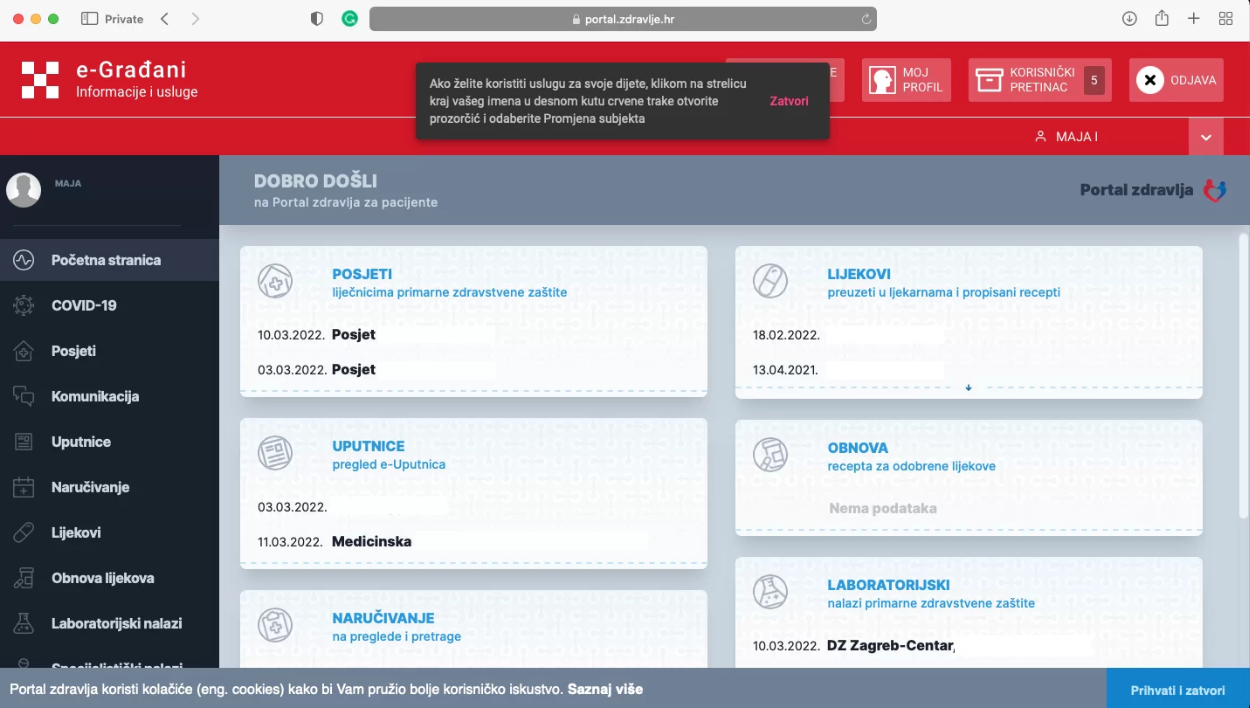
\includegraphics[width=\textwidth]{slike/portalZdravlja.PNG} %veličina u odnosu na širinu linije
			\caption{Snimka zaslona koja prikazuje usluge Portala zdravlja}
		\end{figure}
		
		Sustav bi se u budućnosti mogao nadograditi tako da roditelju dozvoljava mogućnost naručivanja pregleda i biranja termina za sebe i svoju djecu direktno iz aplikacije. Također, sučelje bi se moglo optimizirati time da se poruke mogu filtrirati po vrsti poruke (naručen pregled, nalaz iz laboratorija itd.). Obavljeni pregledi i dijagnoze mogli bi se smjestiti u zasebnom prozoru radi preglednosti. 
		
		\section{Primjeri u \LaTeX u}
		
		\textit{Ovo potpoglavlje izbrisati.}\\

		U nastavku se nalaze različiti primjeri kako koristiti osnovne funkcionalnosti \LaTeX a koje su potrebne za izradu dokumentacije. Za dodatnu pomoć obratiti se asistentu na projektu ili potražiti upute na sljedećim web sjedištima:
		\begin{itemize}
			\item Upute za izradu diplomskog rada u \LaTeX u - \url{https://www.fer.unizg.hr/_download/repository/LaTeX-upute.pdf}
			\item \LaTeX\ projekt - \url{https://www.latex-project.org/help/}
			\item StackExchange za Tex - \url{https://tex.stackexchange.com/}\\
		
		\end{itemize} 	


		
		\noindent \underbar{podcrtani tekst}, \textbf{podebljani tekst}, 	\textit{nagnuti tekst}\\
		\noindent \normalsize primjer \large primjer \Large primjer \LARGE {primjer} \huge {primjer} \Huge primjer \normalsize
				
		\begin{packed_item}
			
			\item  primjer
			\item  primjer
			\item  primjer
			\item[] \begin{packed_enum}
				\item primjer
				\item[] \begin{packed_enum}
					\item[1.a] primjer
					\item[b] primjer
				\end{packed_enum}
				\item primjer
			\end{packed_enum}
			
		\end{packed_item}
		
		\noindent primjer url-a: \url{https://www.fer.unizg.hr/predmet/proinz/projekt}
		
		\noindent posebni znakovi: \# \$ \% \& \{ \} \_ 
		$|$ $<$ $>$ 
		\^{} 
		\~{} 
		$\backslash$ 
		
		
		\begin{longtblr}[
			label=none,
			entry=none
			]{
				width = \textwidth,
				colspec={|X[8,l]|X[8, l]|X[16, l]|}, 
				rowhead = 1,
			} %definicija širine tablice, širine stupaca, poravnanje i broja redaka naslova tablice
			\hline \SetCell[c=3]{c}{\textbf{naslov unutar tablice}}	 \\ \hline[3pt]
			\SetCell{LightGreen}IDKorisnik & INT	&  	Lorem ipsum dolor sit amet, consectetur adipiscing elit, sed do eiusmod  	\\ \hline
			korisnickoIme	& VARCHAR &   	\\ \hline 
			email & VARCHAR &   \\ \hline 
			ime & VARCHAR	&  		\\ \hline 
			\SetCell{LightBlue} primjer	& VARCHAR &   	\\ \hline 
		\end{longtblr}
		

		\begin{longtblr}[
				caption = {Naslov s referencom izvan tablice},
				entry = {Short Caption},
			]{
				width = \textwidth, 
				colspec = {|X[8,l]|X[8,l]|X[16,l]|}, 
				rowhead = 1,
			}
			\hline
			\SetCell{LightGreen}IDKorisnik & INT	&  	Lorem ipsum dolor sit amet, consectetur adipiscing elit, sed do eiusmod  	\\ \hline
			korisnickoIme	& VARCHAR &   	\\ \hline 
			email & VARCHAR &   \\ \hline 
			ime & VARCHAR	&  		\\ \hline 
			\SetCell{LightBlue} primjer	& VARCHAR &   	\\ \hline 
		\end{longtblr}
	


		
		
		%unos slike
		\begin{figure}[H]
			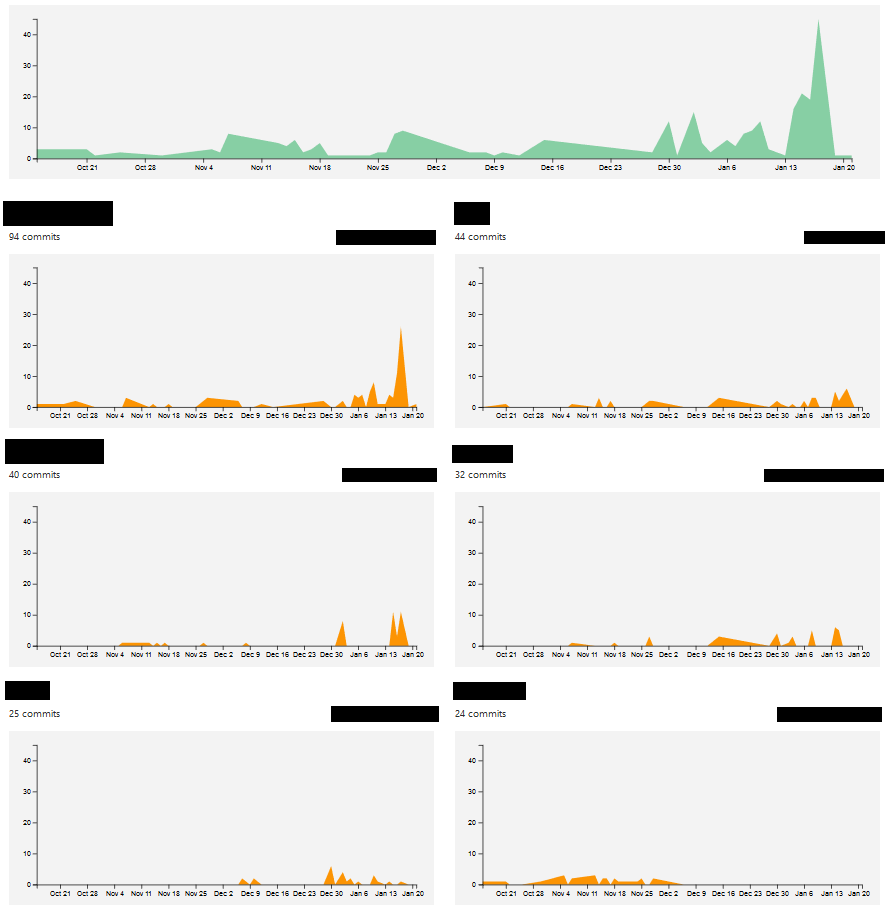
\includegraphics[scale=0.4]{slike/aktivnost.PNG} %veličina slike u odnosu na originalnu datoteku i pozicija slike
			\centering
			\caption{Primjer slike s potpisom}
			\label{fig:promjene}
		\end{figure}
		
		\begin{figure}[H]
			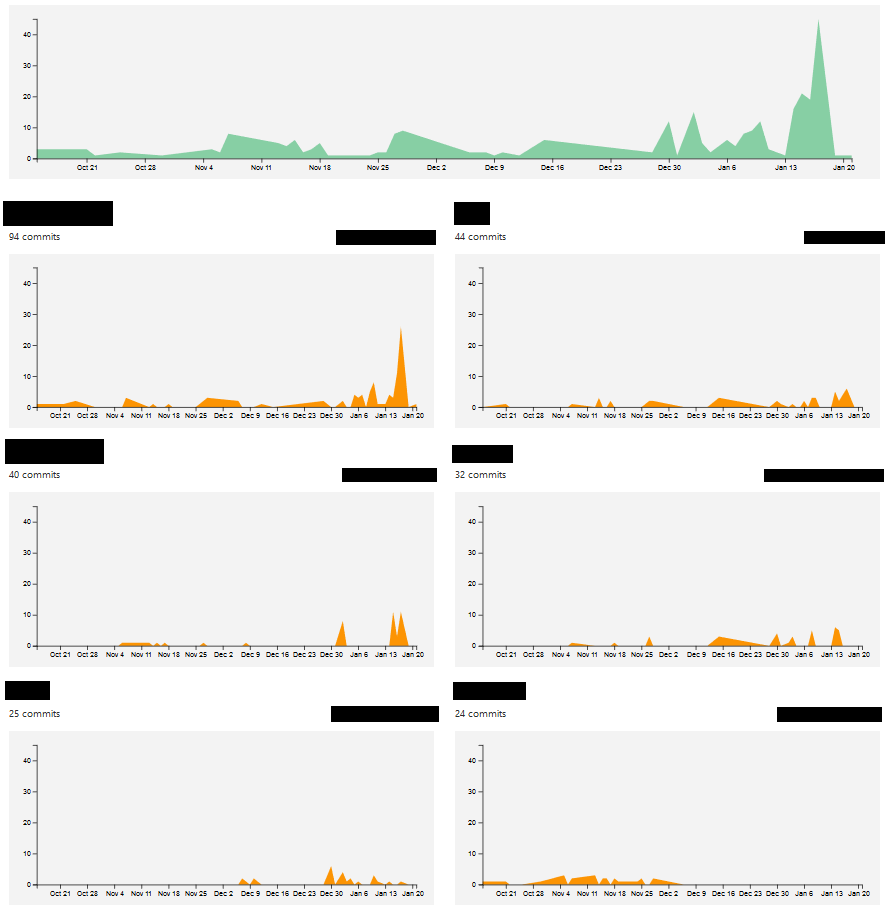
\includegraphics[width=\textwidth]{slike/aktivnost.PNG} %veličina u odnosu na širinu linije
			\caption{Primjer slike s potpisom 2}
			\label{fig:promjene2} %label mora biti drugaciji za svaku sliku
		\end{figure}
		
		Referenciranje slike \ref{fig:promjene2} u tekstu.
		
		\eject
		
	
	\chapter{Specifikacija programske potpore}
		
	\section{Funkcionalni zahtjevi}
			
			\textbf{\textit{dio 1. revizije}}\\
			
			\textit{Navesti \textbf{dionike} koji imaju \textbf{interes u ovom sustavu} ili  \textbf{su nositelji odgovornosti}. To su prije svega korisnici, ali i administratori sustava, naručitelji, razvojni tim.}\\
				
			\textit{Navesti \textbf{aktore} koji izravno \textbf{koriste} ili \textbf{komuniciraju sa sustavom}. Oni mogu imati inicijatorsku ulogu, tj. započinju određene procese u sustavu ili samo sudioničku ulogu, tj. obavljaju određeni posao. Za svakog aktora navesti funkcionalne zahtjeve koji se na njega odnose.}\\
			
			
			\noindent \textbf{Dionici:}
			
			\begin{packed_enum}
				
				\item Roditelji
				\item Zaposlenici u zdravstvenim ustanovama
					\begin{packed_enum}
						\item Liječnici obiteljske medicine
						\item Pedijatri
					\end{packed_enum}				
				\item Administrator
				\item Razvojni tim
				
			\end{packed_enum}
			
			\noindent \textbf{Aktori i njihovi funkcionalni zahtjevi:}
			
			
			\begin{packed_enum}
				\item  \underbar{Neregistrirani/neprijavljeni korisnik (inicijator) može:}
				
				\begin{packed_enum}
					
					\item pročitati opis stranice
					\item se registrirati u sustav, za što mu je potreban OIB te lozinka
					\item se prijaviti u sustav, za što mu je potreban OIB te lozinka
					
				\end{packed_enum}
			
				\item  \underbar{Roditelj (inicijator) može:}
				
				\begin{packed_enum}
					
					\item pregledavati i mijenjati svoje osobne podatke na svom profilu (adresu, mail poslodavca)
					\item pregledavati i mijenjati osobne podatke svoje djece na njihovim profilima (adresu, mail škole/vrtića)
					\item pregledavati obavijesti o odobrenom bolovanju od strane liječnika ili poslanoj ispričnici u školu djeteta
					\item učitati nalaz dobiven temeljem usluge u privatnoj ustanovi te za njega zatražiti povratnu informaciju od liječnika ili pedijatra
					\item pregledavati obavijesti o pristiglim nalazima iz laboratorija
					\item pregledavati potvrde o naručivanju na određeni pregled za sebe ili svoju djecu s prikazanom lokacijom pregleda
					\item pregledavati povijest posjeta liječniku i dijagnoze za sebe i svoju djecu
					\item tražiti dodatna pojašnjenja od liječnika ili pedijatra u vezi bilo koje od gore navedenih stavki
				\end{packed_enum}
				
				\item  \underbar{Liječnik obiteljske medicine (inicijator) može:}
				
				\begin{packed_enum}
					
					\item pregledavati popis svih neprijavljenih roditelja i prijaviti ih kod sebe
					\item pregledavati popis pacijenata prijavljenih kod njega (roditelja)
					\item evidentirati pregled pacijenta te događaje na njemu te utvrditi bolest čime se šalje mail poslodavcu
					\item odobriti preporuku za bolovanje za roditelja koju je izdao pedijatar
					\item poslati obavijest roditelju o pristiglom nalazu iz laboratorija
					\item pregledavati nalaze koji su u sustav učitani od strane roditelja te odgovoriti na njih
					\item naručiti pacijenta na specijalistički pregled
					\item odgovoriti na pitanja roditelja
				\end{packed_enum}
				
				\item  \underbar{Pedijatar (inicijator) može:}
				
				\begin{packed_enum}
					
					\item pregledavati popis sve neprijavljene djece i prijaviti ih kod sebe
					\item pregledavati popis sve djece prijavljene kod njega
					\item izdati preporuku za bolovanje roditelju čije je dijete bolesno
					\item evidentirati pregled djeteta te događaje na njemu te utvrditi bolest čime se šalje ispričnica u školu
					\item poslati obavijest roditelju o pristiglom nalazu iz laboratorija
					\item pregledavati nalaze koji su u sustav učitani od strane roditelja te odgovoriti na njih
					\item naručiti dijete na specijalistički pregled
					\item odgovoriti na pitanja roditelja
					
				\end{packed_enum}
				
				\item  \underbar{Administrator (inicijator) može:}
				
				\begin{packed_enum}
					
					\item vidjeti popis svih registriranih korisnika i njihovih osobnih podataka
					\item brisati korisnike
					\item mijenjati osobne podatke pojedinog korisnika
					\item unijeti registre djece i roditelja (za svaku osobu ime, prezime, OIB i adresu)
					\item registriranom roditelju pridijeliti liječnika obiteljske medicine
					\item djetetu pridijeliti pedijatra
					\item registriranog roditelja povezati s djetetom čiji podaci postoje u sustavu
					
				\end{packed_enum}
				
				\item  \underbar{Baza podataka (sudionik):}
				
				\begin{packed_enum}
					
					\item pohranjuje podatke o svim registriranim korisnicima i njihovim ulogama
					\item pohranjuje podatke o svim postojećim porukama
					\item pohranjuje podatke o postojećim ustanovama i pregledima koje je moguće obaviti u svakoj
					
				\end{packed_enum}
				
				
			\end{packed_enum}
			
			\eject 
			
			
				
			\subsection{Obrasci uporabe}
				
				\textbf{\textit{dio 1. revizije}}
				
				\subsubsection{Opis obrazaca uporabe}
					\textit{Funkcionalne zahtjeve razraditi u obliku obrazaca uporabe. Svaki obrazac je potrebno razraditi prema donjem predlošku. Ukoliko u nekom koraku može doći do odstupanja, potrebno je to odstupanje opisati i po mogućnosti ponuditi rješenje kojim bi se tijek obrasca vratio na osnovni tijek.}\\
					

					\noindent \underbar{\textbf{UC1 - Registracija}}
					\begin{packed_item}
	
						\item \textbf{Glavni sudionik: }Korisnik
						\item  \textbf{Cilj:} Stvoriti korisnički račun za pristup sustavu
						\item  \textbf{Sudionici:} Baza podataka
						\item  \textbf{Preduvjet:} Administrator je u bazi podataka unio osnovne informacije o korisniku (ime, prezime, OIB)
						\item  \textbf{Opis osnovnog tijeka:}
						
						\item[] \begin{packed_enum}
	
							\item Korisnik na početnoj stranici stisne na opciju za registraciju.
							\item Korisnik unosi svoj OIB te željenu lozinku
							\item Korisnik prima obavijest o uspješnoj registraciji
						\end{packed_enum}
						
						\item  \textbf{Opis mogućih odstupanja:}
						
						\item[] \begin{packed_item}
	
							\item[2.a] Odabir OIB-a za koji je zabilježeno da se osoba već registrirala u sustav
							\item[] \begin{packed_enum}
								
								\item Sustav obavještava korisnika o neuspjeloj registraciji i prikaže mu poruku greške
								
								
							\end{packed_enum}
							
							
						\end{packed_item}
					\end{packed_item}
					
					\noindent \underbar{\textbf{UC2 - Prijava u sustav}}
					\begin{packed_item}
						
						\item \textbf{Glavni sudionik: }Korisnik
						\item  \textbf{Cilj:} Dobiti pristup korisničkom sučelju
						\item  \textbf{Sudionici:} Baza podataka
						\item  \textbf{Preduvjet:} Korisnik je registriran
						\item  \textbf{Opis osnovnog tijeka:}
						
						\item[] \begin{packed_enum}
							
							\item Korisnik na početnoj stranici stisne na opciju za prijavu u sustav.
							\item Korisnik unosi svoj OIB te odgovarajuću lozinku
							\item Korisnik prima obavijest o uspješnoj prijavi i preusmjeren je na stranicu svog profila
						\end{packed_enum}
						
						\item  \textbf{Opis mogućih odstupanja:}
						
						\item[] \begin{packed_item}
							
							\item[2.a] OIB nije registriran u sustav ili lozinka ne odgovara navedenom OIB-u.
							\item[] \begin{packed_enum}
								
								\item Sustav obavještava korisnika o neuspjeloj prijavi i prikaže mu poruku greške.
		
								
							\end{packed_enum}
							
						\end{packed_item}
					\end{packed_item}
					
					\noindent \underbar{\textbf{UC3 - Pregled opisa aplikacije}}
					\begin{packed_item}
						
						\item \textbf{Glavni sudionik: }Korisnik
						\item  \textbf{Cilj:} Pregledati osnovne informacije o aplikaciji.
						\item  \textbf{Sudionici:} Baza podataka
						\item  \textbf{Preduvjet:} -
						\item  \textbf{Opis osnovnog tijeka:}
						
						\item[] \begin{packed_enum}
							
							\item Korisnik otvori početnu stranicu aplikacije.
							\item Na početnoj stranici se prikazuju opis i svrha aplikacije te se nude opcije registracije i prijave u sustav (ako korisnik nije prijavljen).
						\end{packed_enum}
						
					
					\end{packed_item}
					
					\noindent \underbar{\textbf{UC4.1 - Pregled profila roditelja}}
					\begin{packed_item}
						
						\item \textbf{Glavni sudionik: }Roditelj
						\item  \textbf{Cilj:} Pregledati svoj profil i osobne podatke na njemu
						\item  \textbf{Sudionici:} Baza podataka
						\item  \textbf{Preduvjet:} Roditelj je prijavljen
						\item  \textbf{Opis osnovnog tijeka:}
						
						\item[] \begin{packed_enum}
							
							\item Roditelj na početnoj stranici odabere svoj profil označen natpisom "Moj profil". 
							\item Roditelj odabere opciju "Pregled osobnih podataka".
							\item Aplikacija prikazuje osobne podatke roditelja (ime, prezime, OIB, adresa, mail poslodavca, liječnik obiteljske medicine).
						\end{packed_enum}
						
						
					\end{packed_item}
					
					\noindent \underbar{\textbf{UC4.2 - Pregled profila djeteta}}
					\begin{packed_item}
						
						\item \textbf{Glavni sudionik: }Roditelj
						\item  \textbf{Cilj:} Pregledati profil djeteta i osobne podatke na njemu
						\item  \textbf{Sudionici:} Baza podataka
						\item  \textbf{Preduvjet:} Roditelj je prijavljen, administrator je povezao roditelja s djetetom
						\item  \textbf{Opis osnovnog tijeka:}
						
						\item[] \begin{packed_enum}
							
							\item Roditelj na početnoj stranici odabere profil djeteta čiji profil želi pregledati. 
							\item Roditelj odabere opciju "Pregled osobnih podataka".
							\item Aplikacija prikazuje osobne podatke djeteta (ime, prezime, OIB, adresa, mail škole/vrtića, pedijatar)
						\end{packed_enum}
						
						\item  \textbf{Opis mogućih odstupanja:}
						
						\item[] \begin{packed_item}
							
							\item[1.a] Dijete još nije povezano s roditeljem u sustavu.
							\item[] \begin{packed_enum}
								
								\item Roditelj neće imati opciju pregleda profila tog djeteta.
								
								
							\end{packed_enum}
						
							
						\end{packed_item}
					\end{packed_item}
					
					\noindent \underbar{\textbf{UC5.1 - Promjena osobnih podataka roditelja}}
					\begin{packed_item}
						
						\item \textbf{Glavni sudionik: }Roditelj
						\item  \textbf{Cilj:} Ažurirati osobne podatke koje roditelj smije mijenjati (adresu, mail poslodavca)
						\item  \textbf{Sudionici:} Baza podataka
						\item  \textbf{Preduvjet:} Roditelj je prijavljen
						\item  \textbf{Opis osnovnog tijeka:}
						
						\item[] \begin{packed_enum}
							
							\item Roditelj na početnoj stranici odabere opciju "Moj profil". 
							\item Roditelj odabere opciju "Pregled osobnih podataka".
							\item Na stranici s podacima roditelj bira opciju za promjenu podataka.
							\item Roditelj sprema podatke.
							\item Baza podataka se ažurira.
						\end{packed_enum}
						
						\item  \textbf{Opis mogućih odstupanja:}
						
						\item[] \begin{packed_item}
							
							\item[4.a] Roditelj promijeni svoje osobne podatke ali ne odabere opciju "Spremi promjene".
							\item[] \begin{packed_enum}
								
								\item Sustav neće pohraniti obavljene promjene.
							\end{packed_enum}
							
						\end{packed_item}
					\end{packed_item}
					
					\noindent \underbar{\textbf{UC5.2 - Promjena osobnih podataka djeteta}}
					\begin{packed_item}
						
						\item \textbf{Glavni sudionik: }Roditelj
						\item  \textbf{Cilj:} Ažurirati osobne podatke o djetetu koje roditelj smije mijenjati (adresu, mail škole/vrtića)
						\item  \textbf{Sudionici:} Baza podataka
						\item  \textbf{Preduvjet:} Roditelj je prijavljen, administrator je povezao roditelja s djetetom
						\item  \textbf{Opis osnovnog tijeka:}
						
						\item[] \begin{packed_enum}
							
							\item Roditelj na početnoj stranici bira profil djeteta čije podatke želi promijeniti. 
							\item Roditelj odabere opciju "Pregled osobnih podataka".
							\item Na stranici s podacima djeteta bira opciju za promjenu podataka.
							\item Roditelj sprema podatke.
							\item Baza podataka se ažurira.
						\end{packed_enum}
						
						\item  \textbf{Opis mogućih odstupanja:}
						
						\item[] \begin{packed_item}
							
							\item[4.a] Roditelj promijeni osobne podatke dijeteta ali ne odabere opciju "Spremi promjene".
							\item[] \begin{packed_enum}
								
								\item Sustav neće pohraniti obavljene promjene.
							\end{packed_enum}
							
						\end{packed_item}
					\end{packed_item}
					
					\noindent \underbar{\textbf{UC6.1 - Učitavanje nalaza roditelja u sustav}}
					\begin{packed_item}
						
						\item \textbf{Glavni sudionik: }Roditelj
						\item  \textbf{Cilj:} Učitati postojeći nalaz u sustav i poslati ga liječniku na pregled
						\item  \textbf{Sudionici:} Baza podataka, liječnik obiteljske medicine
						\item  \textbf{Preduvjet:} Roditelj je prijavljen
						\item  \textbf{Opis osnovnog tijeka:}
						
						\item[] \begin{packed_enum}
							
							\item Roditelj na početnoj stranici bira opciju "Moj profil".
							\item Roditelj na svojoj stranici bira opciju "Učitaj nalaz".
							\item Roditelj učita nalaz u sustav i opiše ga ili postavlja pitanje ako to želi.
							\item Roditelj odabere opciju "Pošalji" čime se nalaz šalje liječniku obiteljske medicine.
							\item Baza podataka se ažurira.
						\end{packed_enum}
						
						\item  \textbf{Opis mogućih odstupanja:}
						
						\item[] \begin{packed_item}
							
							\item[4.a] Roditelj učita nalaz ali ne odabere opciju "Pošalji".
							\item[] \begin{packed_enum}
								
								\item Nalaz se neće poslati.
							\end{packed_enum}
							
							
						\end{packed_item}
					\end{packed_item}
					
						\noindent \underbar{\textbf{UC6.2 - Učitavanje nalaza djeteta u sustav}}
					\begin{packed_item}
						
						\item \textbf{Glavni sudionik: }Roditelj
						\item  \textbf{Cilj:} Učitati postojeći nalaz u sustav i poslati ga pedijatru na pregled
						\item  \textbf{Sudionici:} Baza podataka, pedijatar
						\item  \textbf{Preduvjet:} Roditelj je prijavljen, administrator je povezao roditelja s djetetom
						\item  \textbf{Opis osnovnog tijeka:}
						
						\item[] \begin{packed_enum}
							
							\item Roditelj na početnoj stranici bira profil djeteta čiji nalaz želi učitati u sustav.
							\item Roditelj na djetetovoj stranici bira opciju "Ućitaj nalaz".
							\item Roditelj učita nalaz u sustav i opiše ga ili postavlja pitanje ako to želi.
							\item Roditelj odabere opciju "Pošalji" čime se nalaz šalje pedijatru.
							\item Baza podataka se ažurira.
						\end{packed_enum}
						
						\item  \textbf{Opis mogućih odstupanja:}
						
						\item[] \begin{packed_item}
							
							\item[4.a] Roditelj učita nalaz ali ne odabere opciju "Pošalji".
							\item[] \begin{packed_enum}
								
								\item Nalaz se neće poslati.
							\end{packed_enum}
							
							
						\end{packed_item}
					\end{packed_item}
					
						\noindent \underbar{\textbf{UC7.1 - Pregled podataka o naručenom pregledu roditelja}}
					\begin{packed_item}
						
						\item \textbf{Glavni sudionik: }Roditelj
						\item  \textbf{Cilj:} Pregledati podatke o naručenom pregledu za sebe (vrsta pregleda i lokacije na kojima se može obaviti)
						\item  \textbf{Sudionici:} Baza podataka
						\item  \textbf{Preduvjet:} Roditelj je prijavljen, liječnik je naručio roditelja na specijalistički pregled
						\item  \textbf{Opis osnovnog tijeka:}
						
						\item[] \begin{packed_enum}
							
							\item Roditelj na početnoj stranici bira opciju "Moj profil".
							\item Roditelj odabere jednu od obavijesti s naslovom "[NARUČEN PREGLED]".
							\item Nakon odabira neke od odgovarajućih obavijesti, roditelj može vidjeti koja je vrsta pregleda te može na prikazanom OpenStreetMap pregledu vidjeti u kojim najbližim zdravstvenim ustanovama (s obzirom na adresu roditelja) se pregled može obaviti.
						\end{packed_enum}
						
						\item  \textbf{Opis mogućih odstupanja:}
						
						\item[] \begin{packed_item}
							
							\item[3.a] Roditelj nije unio svoju adresu u sustav.
							\item[] \begin{packed_enum}
								
								\item Sustav obavještava roditelja da za prikaz mogućih zdravstvenih institucija na mapi roditelj mora ažurirati podatak o svojoj adresi na svom profilu.
							\end{packed_enum}
							
							
						\end{packed_item}
					\end{packed_item}
					
					\noindent \underbar{\textbf{UC7.2 - Pregled podataka o naručenom pregledu za dijete}}
					\begin{packed_item}
						
						\item \textbf{Glavni sudionik: }Roditelj
						\item  \textbf{Cilj:} Pregledati podatke o naručenom pregledu za dijete (vrsta pregleda i lokacije na kojima se može obaviti)
						\item  \textbf{Sudionici:} Baza podataka
						\item  \textbf{Preduvjet:} Roditelj je prijavljen, administrator je povezao roditelja s djetetom, pedijatar je naručio dijete na specijalistički pregled
						\item  \textbf{Opis osnovnog tijeka:}
						
						\item[] \begin{packed_enum}
							
							\item Roditelj na početnoj stranici bira profil djeteta za koju želi pregledati naručene preglede 
							\item Roditelj odabere jednu od obavijesti s naslovom "[NARUČEN PREGLED]".
							\item Nakon odabira neke od odgovarajućih obavijesti, roditelj može vidjeti koja je vrsta pregleda te može na prikazanom OpenStreetMap pregledu vidjeti u kojim najbližim zdravstvenim ustanovama (s obzirom na adresu roditelja) se pregled može obaviti.
						\end{packed_enum}
						
						\item  \textbf{Opis mogućih odstupanja:}
						
						\item[] \begin{packed_item}
							
							\item[3.a] Roditelj nije unio adresu djeteta u sustav.
							\item[] \begin{packed_enum}
								
								\item Sustav obavještava roditelja da za prikaz mogućih zdravstvenih institucija na mapi roditelj mora ažurirati podatak o adresi djeteta na njegovom profilu.
							\end{packed_enum}
							
							
						\end{packed_item}
					\end{packed_item}
					
					\noindent \underbar{\textbf{UC8 - Pregled podataka o odobrenom bolovanju}}
					\begin{packed_item}
						
						\item \textbf{Glavni sudionik: }Roditelj
						\item  \textbf{Cilj:} Pregledati podatke o odobrenom bolovanju: razlog bolovanja i trajanje bolovanja
						\item  \textbf{Sudionici:} Baza podataka
						\item  \textbf{Preduvjet:} Roditelj je prijavljen, liječnik je odobrio/preporučio bolovanje roditelju
						\item  \textbf{Opis osnovnog tijeka:}
						
						\item[] \begin{packed_enum}
							
							\item Roditelj na početnoj stranici bira opciju "Moj profil".
							\item Roditelj odabere jednu od obavijesti s naslovom "[BOLOVANJE]".
							\item Nakon odabira neke od odgovarajućih obavijesti, roditelj može vidjeti razlog bolovanja (bolest roditelja ili bolest djeteta), trajanje bolovanja te informacija da je odgovarajući mail poslan poslodavcu.
						\end{packed_enum}
						
						\item  \textbf{Opis mogućih odstupanja:}
						
						\item[] \begin{packed_item}
							
							\item[3.a] Roditelj nije unio mail adresu svog poslodavca.
							\item[] \begin{packed_enum}
								
								\item Unutar obavijesti će biti naznačeno da mail nije poslan poslodavcu jer roditelj u sustav nije unio taj mail.
							\end{packed_enum}
							
							
						\end{packed_item}
					\end{packed_item}
					
					
					\noindent \underbar{\textbf{UC9 - Pregled obavijesti o poslanom mailu vrtiću/školi}}
					\begin{packed_item}
						
						\item \textbf{Glavni sudionik: }Roditelj
						\item  \textbf{Cilj:} Pregledati obavijesti o poslanoj ispričnici vrtiću ili školi
						\item  \textbf{Sudionici:} Baza podataka
						\item  \textbf{Preduvjet:} Roditelj je prijavljen, roditelj je na profilu djeteta unio podatak o mail adresi vrtića ili škole, pedijatar je utvrdio bolest djeteta
						\item  \textbf{Opis osnovnog tijeka:}
						
						\item[] \begin{packed_enum}
							
							\item Roditelj na stranici bira profil djeteta za kojeg se žele pregledati poslane ispričnice.
							\item Roditelj odabere jednu od obavijesti s naslovom "[POSLANA ISPRIČNICA]".
							\item Nakon odabira neke od odgovarajućih obavijesti, roditelj može vidjeti na koji mail je poslana ispričnica.
						\end{packed_enum}
						\item  \textbf{Opis mogućih odstupanja:}
						
						\item[] \begin{packed_item}
							
							\item[2.a] Roditelj nije unio mail adresu vrtića/škole na profilu djeteta.
							\item[] \begin{packed_enum}
								
								\item Ispričnica neće biti poslana (a time roditelj neće nikada ni dobiti obavijest o poslanoj ispričnici).
							\end{packed_enum}
							
							
						\end{packed_item}
						
					\end{packed_item}
					
					\noindent \underbar{\textbf{UC10.1 - Pregled obavljenih pregleda i dijagnoza roditelja}}
					\begin{packed_item}
						
						\item \textbf{Glavni sudionik: }Roditelj
						\item  \textbf{Cilj:} Pregledati podatke o prošlim pregledima i dijagnozama
						\item  \textbf{Sudionici:} Baza podataka
						\item  \textbf{Preduvjet:} Roditelj je prijavljen
						\item  \textbf{Opis osnovnog tijeka:}
						
						\item[] \begin{packed_enum}
							
							\item Roditelj na početnoj stranici bira opciju "Moj profil".
							\item Roditelj odabere jednu od obavijesti s naslovom "[OBAVLJENI PREGLED]".
							\item Nakon odabira neke od odgovarajućih obavijesti, roditelj može vidjeti informacije o obavljenom pregledu te dijagnozi.
						\end{packed_enum}
						
						
					\end{packed_item}
					
					\noindent \underbar{\textbf{UC10.2 - Pregled obavljenih pregleda i dijagnoza djeteta}}
					\begin{packed_item}
						
						\item \textbf{Glavni sudionik: }Roditelj
						\item  \textbf{Cilj:} Pregledati podatke o prošlim pregledima i dijagnozama
						\item  \textbf{Sudionici:} Baza podataka
						\item  \textbf{Preduvjet:} Roditelj je prijavljen, administrator je povezao roditelja s djetetom
						\item  \textbf{Opis osnovnog tijeka:}
						
						\item[] \begin{packed_enum}
							
							\item Roditelj na početnoj stranici bira profil djeteta za kojeg želi pregledati prošle preglede.
							\item Roditelj odabere jednu od obavijesti s naslovom "[OBAVLJENI PREGLED]".
							\item Nakon odabira neke od odgovarajućih obavijesti, roditelj može vidjeti informacije o obavljenom pregledu te dijagnozi.
						\end{packed_enum}
						
						
					\end{packed_item}
					
					\noindent \underbar{\textbf{UC11.1 - Traženje dodatnih pojašnjenja od liječnika}}
					\begin{packed_item}
						
						\item \textbf{Glavni sudionik: }Roditelj
						\item  \textbf{Cilj:} Odgovoriti na poruku koju je primio od liječnika
						\item  \textbf{Sudionici:} Baza podataka, liječnik obiteljske medicine
						\item  \textbf{Preduvjet:} Roditelj je prijavljen u sustav, roditelj je prijavljen kod liječnika, liječnik je poslao poruku
						\item  \textbf{Opis osnovnog tijeka:}
						
						\item[] \begin{packed_enum}
							
							\item Roditelj na početnoj stranici odabere opciju "Moj Profil".
							\item Roditelj bira jednu od poruka koju je primio od liječnika.
							\item Roditelj odabere opciju "Odgovori" i sastavlja svoj odgovor.
							\item Roditelj odabere opciju "Pošalji".
						\end{packed_enum}
						
						\item  \textbf{Opis mogućih odstupanja:}
						
						\item[] \begin{packed_item}
							
							\item[4.a] Roditelj nije odabrao opciju "Pošalji".
							\item[] \begin{packed_enum}
								
								\item Odgovor neće biti poslan.
							\end{packed_enum}
							
							
						\end{packed_item}
						
						
					\end{packed_item}
					
						\noindent \underbar{\textbf{UC11.2 - Traženje dodatnih pojašnjenja od pedijatra}}
					\begin{packed_item}
						
						\item \textbf{Glavni sudionik: }Roditelj
						\item  \textbf{Cilj:} Odgovoriti na poruku koju je primio od pedijatra u vezi svog djeteta
						\item  \textbf{Sudionici:} Baza podataka, pedijatar
						\item  \textbf{Preduvjet:} Roditelj je prijavljen u sustav, administrator je povezao dijete s roditeljem, dijete je prijavljeno kod pedijatra, pedijatar je poslao poruku
						\item  \textbf{Opis osnovnog tijeka:}
						
						\item[] \begin{packed_enum}
							
							\item Roditelj na početnoj stranici odabere profil odgovarajućeg djeteta.
							\item Roditelj bira jednu od poruka koju je primio od pedijatra.
							\item Roditelj odabere opciju "Odgovori" i sastavlja svoj odgovor.
							\item Roditelj odabere opciju "Pošalji".
						\end{packed_enum}
						
						\item  \textbf{Opis mogućih odstupanja:}
						
						\item[] \begin{packed_item}
							
							\item[4.a] Roditelj nije odabrao opciju "Pošalji".
							\item[] \begin{packed_enum}
								
								\item Odgovor neće biti poslan.
							\end{packed_enum}
							
							
						\end{packed_item}
						
						
					\end{packed_item}
					
					\noindent \underbar{\textbf{UC12 - Pregled popisa djece prijavljene kod nekog pedijatra}}
					\begin{packed_item}
						
						\item \textbf{Glavni sudionik: }Pedijatar
						\item  \textbf{Cilj:} Pregledati popis djece prijavljene kod njega
						\item  \textbf{Sudionici:} Baza podataka
						\item  \textbf{Preduvjet:} Pedijatar je prijavio djecu kod sebe ili je administrator povezao dijete s pedijatrom
						\item  \textbf{Opis osnovnog tijeka:}
						
						\item[] \begin{packed_enum}
							
							\item Pedijatar nakon prijave na početnoj stranici može vidjeti popis djece prijavljene kod njega.
						\end{packed_enum}
						
						
					\end{packed_item}
					
					\noindent \underbar{\textbf{UC13 - Prijava novog djeteta kod pedijatra}}
					\begin{packed_item}
						
						\item \textbf{Glavni sudionik: }Pedijatar
						\item  \textbf{Cilj:} Pregledati popis neprijavljene djece i prijaviti ih kod sebe
						\item  \textbf{Sudionici:} Baza podataka
						\item  \textbf{Preduvjet:} Administrator je unio podatke o djeci, pedijatar je prijavljen u sustav
						\item  \textbf{Opis osnovnog tijeka:}
						
						\item[] \begin{packed_enum}
							
							\item Pedijatar na početnoj stranici bira opciju "Prijavi novo dijete".
							\item Pedijatar u popisu neprijavljene djece pronalazi dijete koje želi prijaviti kod sebe i odabere opciju "Prijavi".
							\item Dijete se sada nalazi u popisu prijavljene djece na početnoj stranici.
						\end{packed_enum}
						
						
					\end{packed_item}
					
					\noindent \underbar{\textbf{UC14 - Upis podataka o pregledu djeteta obavljenom kod pedijatra i dijagnoza}}
					\begin{packed_item}
						
						\item \textbf{Glavni sudionik: }Pedijatar
						\item  \textbf{Cilj:} Upisati podatak o obavljenom pregledu djeteta
						\item  \textbf{Sudionici:} Baza podataka, roditelj
						\item  \textbf{Preduvjet:} Pedijatar je prijavljen u sustav, dijete je prijavljeno kod pedijatra
						\item  \textbf{Opis osnovnog tijeka:}
						
						\item[] \begin{packed_enum}
							
							\item Pedijatar na početnoj stranici iz popisa djece prijavljene kod njega bira dijete čiji pregled želi unijeti.
							\item Pedijatar bira opciju "Dijagnoza".
							\item Pedijatar opiše pregled i dijagnozu te opcionalno može odabrati šalje li se ispričnica i preporuka za bolovanje roditelja.
							\item Pedijatar bira opciju "Pošalji".
						\end{packed_enum}
						
						\item  \textbf{Opis mogućih odstupanja:}
						
						\item[] \begin{packed_item}
							
							\item[4.a] Pedijatar nije odabrao opciju "Pošalji".
							\item[] \begin{packed_enum}
								
								\item Podaci neće biti upisani.
							\end{packed_enum}
							
							
						\end{packed_item}
						
						
					\end{packed_item}
					
					
					\noindent \underbar{\textbf{UC15 - Izdavanje preporuke za bolovanje za roditelja bolesnog djeteta}}
					\begin{packed_item}
						
						\item \textbf{Glavni sudionik: }Pedijatar
						\item  \textbf{Cilj:} Izdati preporuku za bolovanje roditelju bolesnog djeteta
						\item  \textbf{Sudionici:} Baza podataka, roditelj, liječnik obiteljske medicine
						\item  \textbf{Preduvjet:} Pedijatar je prijavljen u sustav, dijete je prijavljeno kod pedijatra
						\item  \textbf{Opis osnovnog tijeka:}
						
						\item[] \begin{packed_enum}
							
							\item Pedijatar na početnoj stranici iz popisa djece prijavljene kod njega bira dijete čijem roditelju želi izdati preporuku za bolovanje.
							\item Pedijatar bira opciju "Dijagnoza".
							\item Pedijatar opiše razlog izdavanja preporuke te bira opciju "Preporuka za bolovanje roditelja" i opciju "Ispričnica školi/vrtiću".
							\item Pedijatar bira opciju "Pošalji".
						\end{packed_enum}
						
						\item  \textbf{Opis mogućih odstupanja:}
						
						\item[] \begin{packed_item}
							
							\item[4.a] Pedijatar nije odabrao opciju "Pošalji".
							\item[] \begin{packed_enum}
								
								\item Preporuka neće biti upisana.
							\end{packed_enum}
							
							
						\end{packed_item}
						
						
					\end{packed_item}
					
					\noindent \underbar{\textbf{UC16 - Slanje nalaza iz laboratorija djeteta}}
					\begin{packed_item}
						
						\item \textbf{Glavni sudionik: }Pedijatar
						\item  \textbf{Cilj:} Roditelju djeteta poslati laboratorijski nalaz djeteta
						\item  \textbf{Sudionici:} Baza podataka, roditelj
						\item  \textbf{Preduvjet:} Pedijatar je prijavljen u sustav, dijete je prijavljeno kod pedijatra
						\item  \textbf{Opis osnovnog tijeka:}
						
						\item[] \begin{packed_enum}
							
							\item Pedijatar na početnoj stranici iz popisa djece prijavljene kod njega bira dijete čiji pregled želi unijeti.
							\item Pedijatar bira opciju "Nalaz iz laboratorija".
							\item Pedijatar opiše nalaz te može priložiti dokument biranjem opcije "Prilog" te opcionalno može odabrati šalje li se ispričnica i preporuka za bolovanje roditelja.
							\item Pedijatar bira opciju "Pošalji".
						\end{packed_enum}
						
						\item  \textbf{Opis mogućih odstupanja:}
						
						\item[] \begin{packed_item}
							
							\item[4.a] Pedijatar nije odabrao opciju "Pošalji".
							\item[] \begin{packed_enum}
								
								\item Nalaz neće biti poslan.
							\end{packed_enum}
							
							
						\end{packed_item}
						
						
					\end{packed_item}
					
					\noindent \underbar{\textbf{UC17 - Pregled učitanih nalaza djeteta od strane roditelja}}
					\begin{packed_item}
						
						\item \textbf{Glavni sudionik: }Pedijatar
						\item  \textbf{Cilj:} Pregledati nalaze djeteta koje su roditelji učitali u sustav
						\item  \textbf{Sudionici:} Baza podataka
						\item  \textbf{Preduvjet:} Pedijatar je prijavljen u sustav, dijete je prijavljeno kod pedijatra, pedijatar je primio obavijest o učitanom nalazu
						\item  \textbf{Opis osnovnog tijeka:}
						
						\item[] \begin{packed_enum}
							
							\item Pedijatar na početnoj stranici iz popisa djece prijavljene kod njega bira dijete čije nalaze želi vidjeti.
							\item Pedijatar bira jednu od obavijesti s naslovom [UČITAN NALAZ].
							\item Pedijatar može pregledati nalaz te dodatna pitanja ili informacije koje je roditelj priložio.
						\end{packed_enum}
						
						
					\end{packed_item}
					
					\noindent \underbar{\textbf{UC18 - Davanje povratne informacije roditelju o bolesti djeteta}}
					\begin{packed_item}
						
						\item \textbf{Glavni sudionik: }Pedijatar
						\item  \textbf{Cilj:} Odgovoriti na poruku roditelja u vezi djeteta
						\item  \textbf{Sudionici:} Baza podataka, roditelj
						\item  \textbf{Preduvjet:} Pedijatar je prijavljen u sustav, dijete je prijavljeno kod pedijatra, pedijatar je primio obavijest o učitanom nalazu
						\item  \textbf{Opis osnovnog tijeka:}
						
						\item[] \begin{packed_enum}
							
							\item Pedijatar na početnoj stranici iz popisa djece prijavljene kod njega bira dijete za koje postoji poruka poslana od strane roditelja koja očekuje odgovor.
							\item Pedijatar odabere jednu od poruka koju je poslao roditelj
							\item Pedijatar odabere opciju "Odgovori" i sastavlja svoj odgovor.
							\item Pedijatar odabere opciju "Pošalji".
						\end{packed_enum}
						
						\item  \textbf{Opis mogućih odstupanja:}
						
						\item[] \begin{packed_item}
							
							\item[4.a] Pedijatar nije odabrao opciju "Pošalji".
							\item[] \begin{packed_enum}
								
								\item Odgovor neće biti poslan.
							\end{packed_enum}
							
							
						\end{packed_item}
						
						
					\end{packed_item}
					
					\noindent \underbar{\textbf{UC19 - Naručivanje djeteta na specijalistički pregled}}
					\begin{packed_item}
						
						\item \textbf{Glavni sudionik: }Pedijatar
						\item  \textbf{Cilj:} Naručiti dijete na specijalistički pregled
						\item  \textbf{Sudionici:} Baza podataka
						\item  \textbf{Preduvjet:} Pedijatar je prijavljen u sustav, dijete je prijavljeno kod pedijatra
						\item  \textbf{Opis osnovnog tijeka:}
						
						\item[] \begin{packed_enum}
							
							\item Pedijatar na početnoj stranici iz popisa djece prijavljene kod njega bira dijete koje želi naručiti na specijalistički pregled.
							\item Pedijatar odabere opciju "Naručivanje specijalističkog pregleda.
							\item Pedijatar odabere vrstu pregleda te dodaje napomenu ako to želi.
							\item Pedijatar odabere opciju "Pošalji".
						\end{packed_enum}
						
						\item  \textbf{Opis mogućih odstupanja:}
						
						\item[] \begin{packed_item}
							
							\item[4.a] Pedijatar nije odabrao opciju "Pošalji".
							\item[] \begin{packed_enum}
								
								\item Dijete neće biti naručeno.
							\end{packed_enum}
							
							
						\end{packed_item}
						
						
					\end{packed_item}
					
					\noindent \underbar{\textbf{UC20 - Pregled popisa roditelja prijavljenih kod nekog liječnika obiteljske medicine}}
					\begin{packed_item}
						
						\item \textbf{Glavni sudionik: }Liječnik obiteljske medicine
						\item  \textbf{Cilj:} Pregledati popis roditelja prijavljenih kod njega
						\item  \textbf{Sudionici:} Baza podataka
						\item  \textbf{Preduvjet:} Liječnik je prijavio roditelja kod sebe ili je administrator povezao roditelja s liječnikom
						\item  \textbf{Opis osnovnog tijeka:}
						
						\item[] \begin{packed_enum}
							
							\item Liječnik nakon prijave na početnoj stranici može vidjeti popis roditelja (pacijenata) prijavljenih kod njega.
						\end{packed_enum}
						
						
					\end{packed_item}
					
					\noindent \underbar{\textbf{UC21 - Prijava novog roditelja kod liječnika}}
					\begin{packed_item}
						
						\item \textbf{Glavni sudionik: }Liječnik obiteljske medicine
						\item  \textbf{Cilj:} Pregledati popis neprijavljenih roditelja i prijaviti ih kod sebe
						\item  \textbf{Sudionici:} Baza podataka, roditelj
						\item  \textbf{Preduvjet:} Administrator je unio podatke o roditeljima, liječnik je prijavljen u sustav
						\item  \textbf{Opis osnovnog tijeka:}
						
						\item[] \begin{packed_enum}
							
							\item Liiečnik na početnoj stranici bira opciju "Prijavi novog pacijenta".
							\item Liječnik u popisu neprijavljenih roditelja pronalazi osobu koje želi prijaviti kod sebe i odabere opciju "Prijavi".
							\item Roditelj se sada nalazi u popisu prijavljenih pacijenata na početnoj stranici.
						\end{packed_enum}
						
						
					\end{packed_item}
					
					\noindent \underbar{\textbf{UC22 - Upis podataka o pregledu roditelja obavljenom kod liječnika i dijagnoza}}
					\begin{packed_item}
						
						\item \textbf{Glavni sudionik: }Liječnik obiteljske medicine
						\item  \textbf{Cilj:} Upisati podatak o obavljenom pregledu roditelja
						\item  \textbf{Sudionici:} Baza podataka, roditelj
						\item  \textbf{Preduvjet:} Liječnik je prijavljen u sustav, roditelj je prijavljeno kod liječnika
						\item  \textbf{Opis osnovnog tijeka:}
						
						\item[] \begin{packed_enum}
							
							\item Liječnik na početnoj stranici iz popisa roditelja prijavljenih kod njega bira roditelja čiji pregled želi unijeti.
							\item Liječnik bira opciju "Dijagnoza".
							\item Liječnik opiše pregled i dijagnozu te opcionalno može odabrati izdaje li se bolovanje za roditelja.
							\item Liječnik bira opciju "Pošalji".
						\end{packed_enum}
						
						\item  \textbf{Opis mogućih odstupanja:}
						
						\item[] \begin{packed_item}
							
							\item[4.a] Liječnik nije odabrao opciju "Pošalji".
							\item[] \begin{packed_enum}
								
								\item Pregled neće biti upisan.
							\end{packed_enum}
							
							
						\end{packed_item}
						
						
					\end{packed_item}
					
					
					
					\noindent \underbar{\textbf{UC23 - Odobrenje preporuke za bolovanje za roditelja bolesnog djeteta}}
					\begin{packed_item}
						
						\item \textbf{Glavni sudionik: }Liječnik obiteljske medicine
						\item  \textbf{Cilj:} Odobriti preporuku za bolovanje roditelju bolesnog djeteta koju je izdao pedijatar
						\item  \textbf{Sudionici:} Baza podataka, roditelj
						\item  \textbf{Preduvjet:} Liječnik je prijavljen u sustav, pedijatar je izdao preporuku za bolovanje roditelju zbog bolesti djeteta
						\item  \textbf{Opis osnovnog tijeka:}
						
						\item[] \begin{packed_enum}
							
							\item Liječnik na početnoj stranici iz popisa roditelja prijavljenih kod njega bira roditelja za kojeg želi odobriti preporuku za bolovanje.
							\item Liječnik bira poruku s naslovom [PREPORUKA BOLOVANJA].
							\item Liječnik u novootvorenom prozoru bira opciju "Omogući bolovanje".
						\end{packed_enum}
						
						
						
					\end{packed_item}
					
					
					\noindent \underbar{\textbf{UC24 - Propisivanje bolovanja za bolesnog roditelja}}
					\begin{packed_item}
						
						\item \textbf{Glavni sudionik: }Liječnik obiteljske medicine
						\item  \textbf{Cilj:} Izdati preporuku za bolovanje bolesnom roditelju
						\item  \textbf{Sudionici:} Baza podataka, roditelj
						\item  \textbf{Preduvjet:} Liječnik je prijavljen u sustav, roditelj je prijavljen kod pedijatra
						\item  \textbf{Opis osnovnog tijeka:}
						
						\item[] \begin{packed_enum}
							
							\item Liječnik na početnoj stranici iz popisa roditelja prijavljenih kod njega bira roditelja kojem želi propisati bolovanje.
							\item Liječnik bira opciju "Dijagnoza".
							\item Liječnik opiše razlog propisivanja bolovanja te bira opciju "Bolovanje".
							\item Liječnik bira opciju "Pošalji".
						\end{packed_enum}
						
						\item  \textbf{Opis mogućih odstupanja:}
						
						\item[] \begin{packed_item}
							
							\item[4.a] Liječnik nije odabrao opciju "Pošalji".
							\item[] \begin{packed_enum}
								
								\item Preporuka za bolovanje neće biti izdana.
							\end{packed_enum}
							
							
						\end{packed_item}
						
						
					\end{packed_item}
					
					\noindent \underbar{\textbf{UC25 - Slanje nalaza iz laboratorija roditelja}}
					\begin{packed_item}
						
						\item \textbf{Glavni sudionik: }Liječnik obiteljske medicine
						\item  \textbf{Cilj:} Roditelju poslati njegov laboratorijski nalaz 
						\item  \textbf{Sudionici:} Baza podataka, roditelj
						\item  \textbf{Preduvjet:} Liječnik je prijavljen u sustav, roditelj je prijavljen kod liječnika
						\item  \textbf{Opis osnovnog tijeka:}
						
						\item[] \begin{packed_enum}
							
							\item Liječnik na početnoj stranici iz popisa roditelja prijavljenih kod njega bira roditelja čiji nalaz želi unijeti.
							\item Liječnik bira opciju "Nalaz iz laboratorija".
							\item Liječnik opiše nalaz te može priložiti dokument biranjem opcije "Prilog" te opcionalno može odabrati i opciju za izdavanje bolovanja.
							\item Liječnik bira opciju "Pošalji".
						\end{packed_enum}
						
						\item  \textbf{Opis mogućih odstupanja:}
						
						\item[] \begin{packed_item}
							
							\item[4.a] Liječnik nije odabrao opciju "Pošalji".
							\item[] \begin{packed_enum}
								
								\item Nalaz neće biti poslan.
							\end{packed_enum}
							
							
						\end{packed_item}
						
						
					\end{packed_item}
					
					\noindent \underbar{\textbf{UC26 - Pregled učitanih nalaza roditelja}}
					\begin{packed_item}
						
						\item \textbf{Glavni sudionik: }Liječnik obiteljske medicine
						\item  \textbf{Cilj:} Pregledati nalaze koje je pojedini pacijent (roditelj) učitao u sustav
						\item  \textbf{Sudionici:} Baza podataka
						\item  \textbf{Preduvjet:} Liječnik je prijavljen u sustav, roditelj je prijavljen kod liječnika, liječnik je primio obavijest o učitanom nalazu
						\item  \textbf{Opis osnovnog tijeka:}
						
						\item[] \begin{packed_enum}
							
							\item Liječnik na početnoj stranici iz popisa roditelja prijavljenih kod njega bira onog čije nalaze želi vidjeti.
							\item Liječnik bira jednu od obavijesti s naslovom [UČITAN NALAZ].
							\item Liječnik može pregledati nalaz te dodatna pitanja ili informacije koje je roditelj priložio.
						\end{packed_enum}
						
						
					\end{packed_item}
					
					\noindent \underbar{\textbf{UC27 - Davanje povratne informacije roditelju}}
					\begin{packed_item}
						
						\item \textbf{Glavni sudionik: }Liječnik obiteljske medicine
						\item  \textbf{Cilj:} Odgovoriti na poruku koju je poslao pacijent (roditelj)
						\item  \textbf{Sudionici:} Baza podataka, roditelj
						\item  \textbf{Preduvjet:} Liječnik je prijavljen u sustav, roditelj je prijavljen kod liječnika, liječnik je primio poruku
						\item  \textbf{Opis osnovnog tijeka:}
						
						\item[] \begin{packed_enum}
							
							\item Liječnik na početnoj stranici iz popisa roditelja prijavljenih kod njega bira roditelja na čiju poruku želi odgovoriti.
							\item Liječnik bira jednu od poruka koju je primio od roditelja-
							\item Liječnik odabere opciju "Odgovori" i sastavlja svoj odgovor.
							\item Liječnik odabere opciju "Pošalji".
						\end{packed_enum}
						
						\item  \textbf{Opis mogućih odstupanja:}
						
						\item[] \begin{packed_item}
							
							\item[3.a] Liječnik nije odabrao opciju "Pošalji".
							\item[] \begin{packed_enum}
								
								\item Odgovor neće biti poslan.
							\end{packed_enum}
							
							
						\end{packed_item}
						
						
					\end{packed_item}
					
					\noindent \underbar{\textbf{UC28 - Naručivanje roditelja na specijalistički pregled}}
					\begin{packed_item}
						
						\item \textbf{Glavni sudionik: }Liječnik obiteljske medicine
						\item  \textbf{Cilj:} Naručiti roditelja na specijalistički pregled
						\item  \textbf{Sudionici:} Baza podataka, roditelj
						\item  \textbf{Preduvjet:} Liječnik je prijavljen u sustav, roditelj je prijavljen kod liječnika
						\item  \textbf{Opis osnovnog tijeka:}
						
						\item[] \begin{packed_enum}
							
							\item Liječnik na početnoj stranici iz popisa roditelja prijavljenih kod njega bira roditelja kojeg želi naručiti na specijalistički pregled.
							\item Liječnik odabere opciju "Naručivanje specijalističkog pregleda.
							\item Liječnik odabere vrstu pregleda te dodaje napomenu ako to želi.
							\item Liječnik odabere opciju "Pošalji".
						\end{packed_enum}
						
						\item  \textbf{Opis mogućih odstupanja:}
						
						\item[] \begin{packed_item}
							
							\item[4.a] Liječnik nije odabrao opciju "Pošalji".
							\item[] \begin{packed_enum}
								
								\item Roditelj neće biti naručen na pregled.
							\end{packed_enum}
							
							
						\end{packed_item}
						
						
					\end{packed_item}
					
						\noindent \underbar{\textbf{UC29 - Pregled svih postojećih osoba upisanih u sustav}}
					\begin{packed_item}
						
						\item \textbf{Glavni sudionik: }Administrator
						\item  \textbf{Cilj:} Pregledati sve roditelje i djecu koji su već upisani u sustav
						\item  \textbf{Sudionici:} Baza podataka
						\item  \textbf{Preduvjet:} Administrator je prijavljen
						\item  \textbf{Opis osnovnog tijeka:}
						
						\item[] \begin{packed_enum}
							
							\item Administrator nakon prijave u sustav ima pregled liste svih osoba prijavljenih u sustav (ime, prezime, OIB).
						\end{packed_enum}
						
						\item  \textbf{Opis mogućih odstupanja:}
						
						\item[] \begin{packed_item}
							
							\item[4.a] Administrator još nije nijednu osobu prijavio u sustav.
							\item[] \begin{packed_enum}
								
								\item Lista prijavljenih je prazna.
							\end{packed_enum}
							
							
						\end{packed_item}
						
						
					\end{packed_item}
					
					
					\noindent \underbar{\textbf{UC30.1 - Prijavljivanje novog roditelja  u sustav}}
					\begin{packed_item}
						
						\item \textbf{Glavni sudionik: }Administrator
						\item  \textbf{Cilj:} Prijaviti novu osobu u sustav
						\item  \textbf{Sudionici:} Baza podataka
						\item  \textbf{Preduvjet:} Administrator je prijavljen
						\item  \textbf{Opis osnovnog tijeka:}
						
						\item[] \begin{packed_enum}
							
							\item Administrator na početnoj stranici bira opciju "Dodaj roditelja".
							\item Administrator upisuje ime, prezime, OIB i datum rođenja roditelja.
							\item Administrator odabere opciju "Dodaj".
						\end{packed_enum}
						
						\item  \textbf{Opis mogućih odstupanja:}
						
						\item[] \begin{packed_item}
							
							\item[3.a] Administrator ne odabere opciju "Dodaj".
							\item[] \begin{packed_enum}
								
								\item Roditelj neće biti dodan.
							\end{packed_enum}
							
							
						\end{packed_item}
						
						
					\end{packed_item}
					
					\noindent \underbar{\textbf{UC30.2 - Prijavljivanje novog djeteta  u sustav}}
					\begin{packed_item}
						
						\item \textbf{Glavni sudionik: }Administrator
						\item  \textbf{Cilj:} Prijaviti novu osobu u sustav
						\item  \textbf{Preduvjet:} Administrator je prijavljen, roditelj djeteta kojeg dodajemo već postoji u sustavu.
						\item  \textbf{Sudionici:} Baza podataka
						\item  \textbf{Opis osnovnog tijeka:}
						
						\item[] \begin{packed_enum}
							
							\item Administrator na početnoj stranici bira opciju "Dodaj dijete".
							\item Administrator upisuje ime, prezime, OIB djeteta, OIB roditelja (iz liste postojećih OIB-a roditelja u sustavu) i datum rođenja djeteta.
							\item Administrator odabere opciju "Dodaj".
						\end{packed_enum}
						
						\item  \textbf{Opis mogućih odstupanja:}
						
						\item[] \begin{packed_item}
							
							
							\item[3.a] Administrator ne odabere opciju "Dodaj".
							\item[] \begin{packed_enum}
								
								\item Dijete neće biti dodano.
							\end{packed_enum}
							
							
						\end{packed_item}
						
						
					\end{packed_item}
					
					\noindent \underbar{\textbf{UC31 - Mijenjanje osobnih podataka osobe prijavljene u sustav}}
					\begin{packed_item}
						
						\item \textbf{Glavni sudionik: }Administrator
						\item  \textbf{Cilj:} Prijaviti novu osobu u sustav
						\item  \textbf{Sudionici:} Baza podataka
						\item  \textbf{Preduvjet:} Administrator je prijavljen, osoba je prijavljena u sustavu
						\item  \textbf{Opis osnovnog tijeka:}
						
						\item[] \begin{packed_enum}
							
							\item Administrator na početnoj stranici bira iz liste prijavljenih osobu čije osobne podatke želi promijeniti.
							\item Administrator u novootvorenom prozoru može mijenjati podatke osobe: ime, prezime, OIB, adresu, mail poslodavca/vrtića te može osobi pridijeliti liječnika/pedijatra.
							\item Administrator odabere opciju "Pohrani".
						\end{packed_enum}
						
						\item  \textbf{Opis mogućih odstupanja:}
						
						\item[] \begin{packed_item}
							
							\item[3.a] Administrator ne odabere opciju "Pohrani".
							\item[] \begin{packed_enum}
								
								\item Promjene neće biti pohranjene.
							\end{packed_enum}
							
							
						\end{packed_item}
						
						
					\end{packed_item}
					
					
				
					
				\subsubsection{Dijagrami obrazaca uporabe}
					\textbf{\textit{dio 1. revizije}}\\
						\begin{figure}[H]
						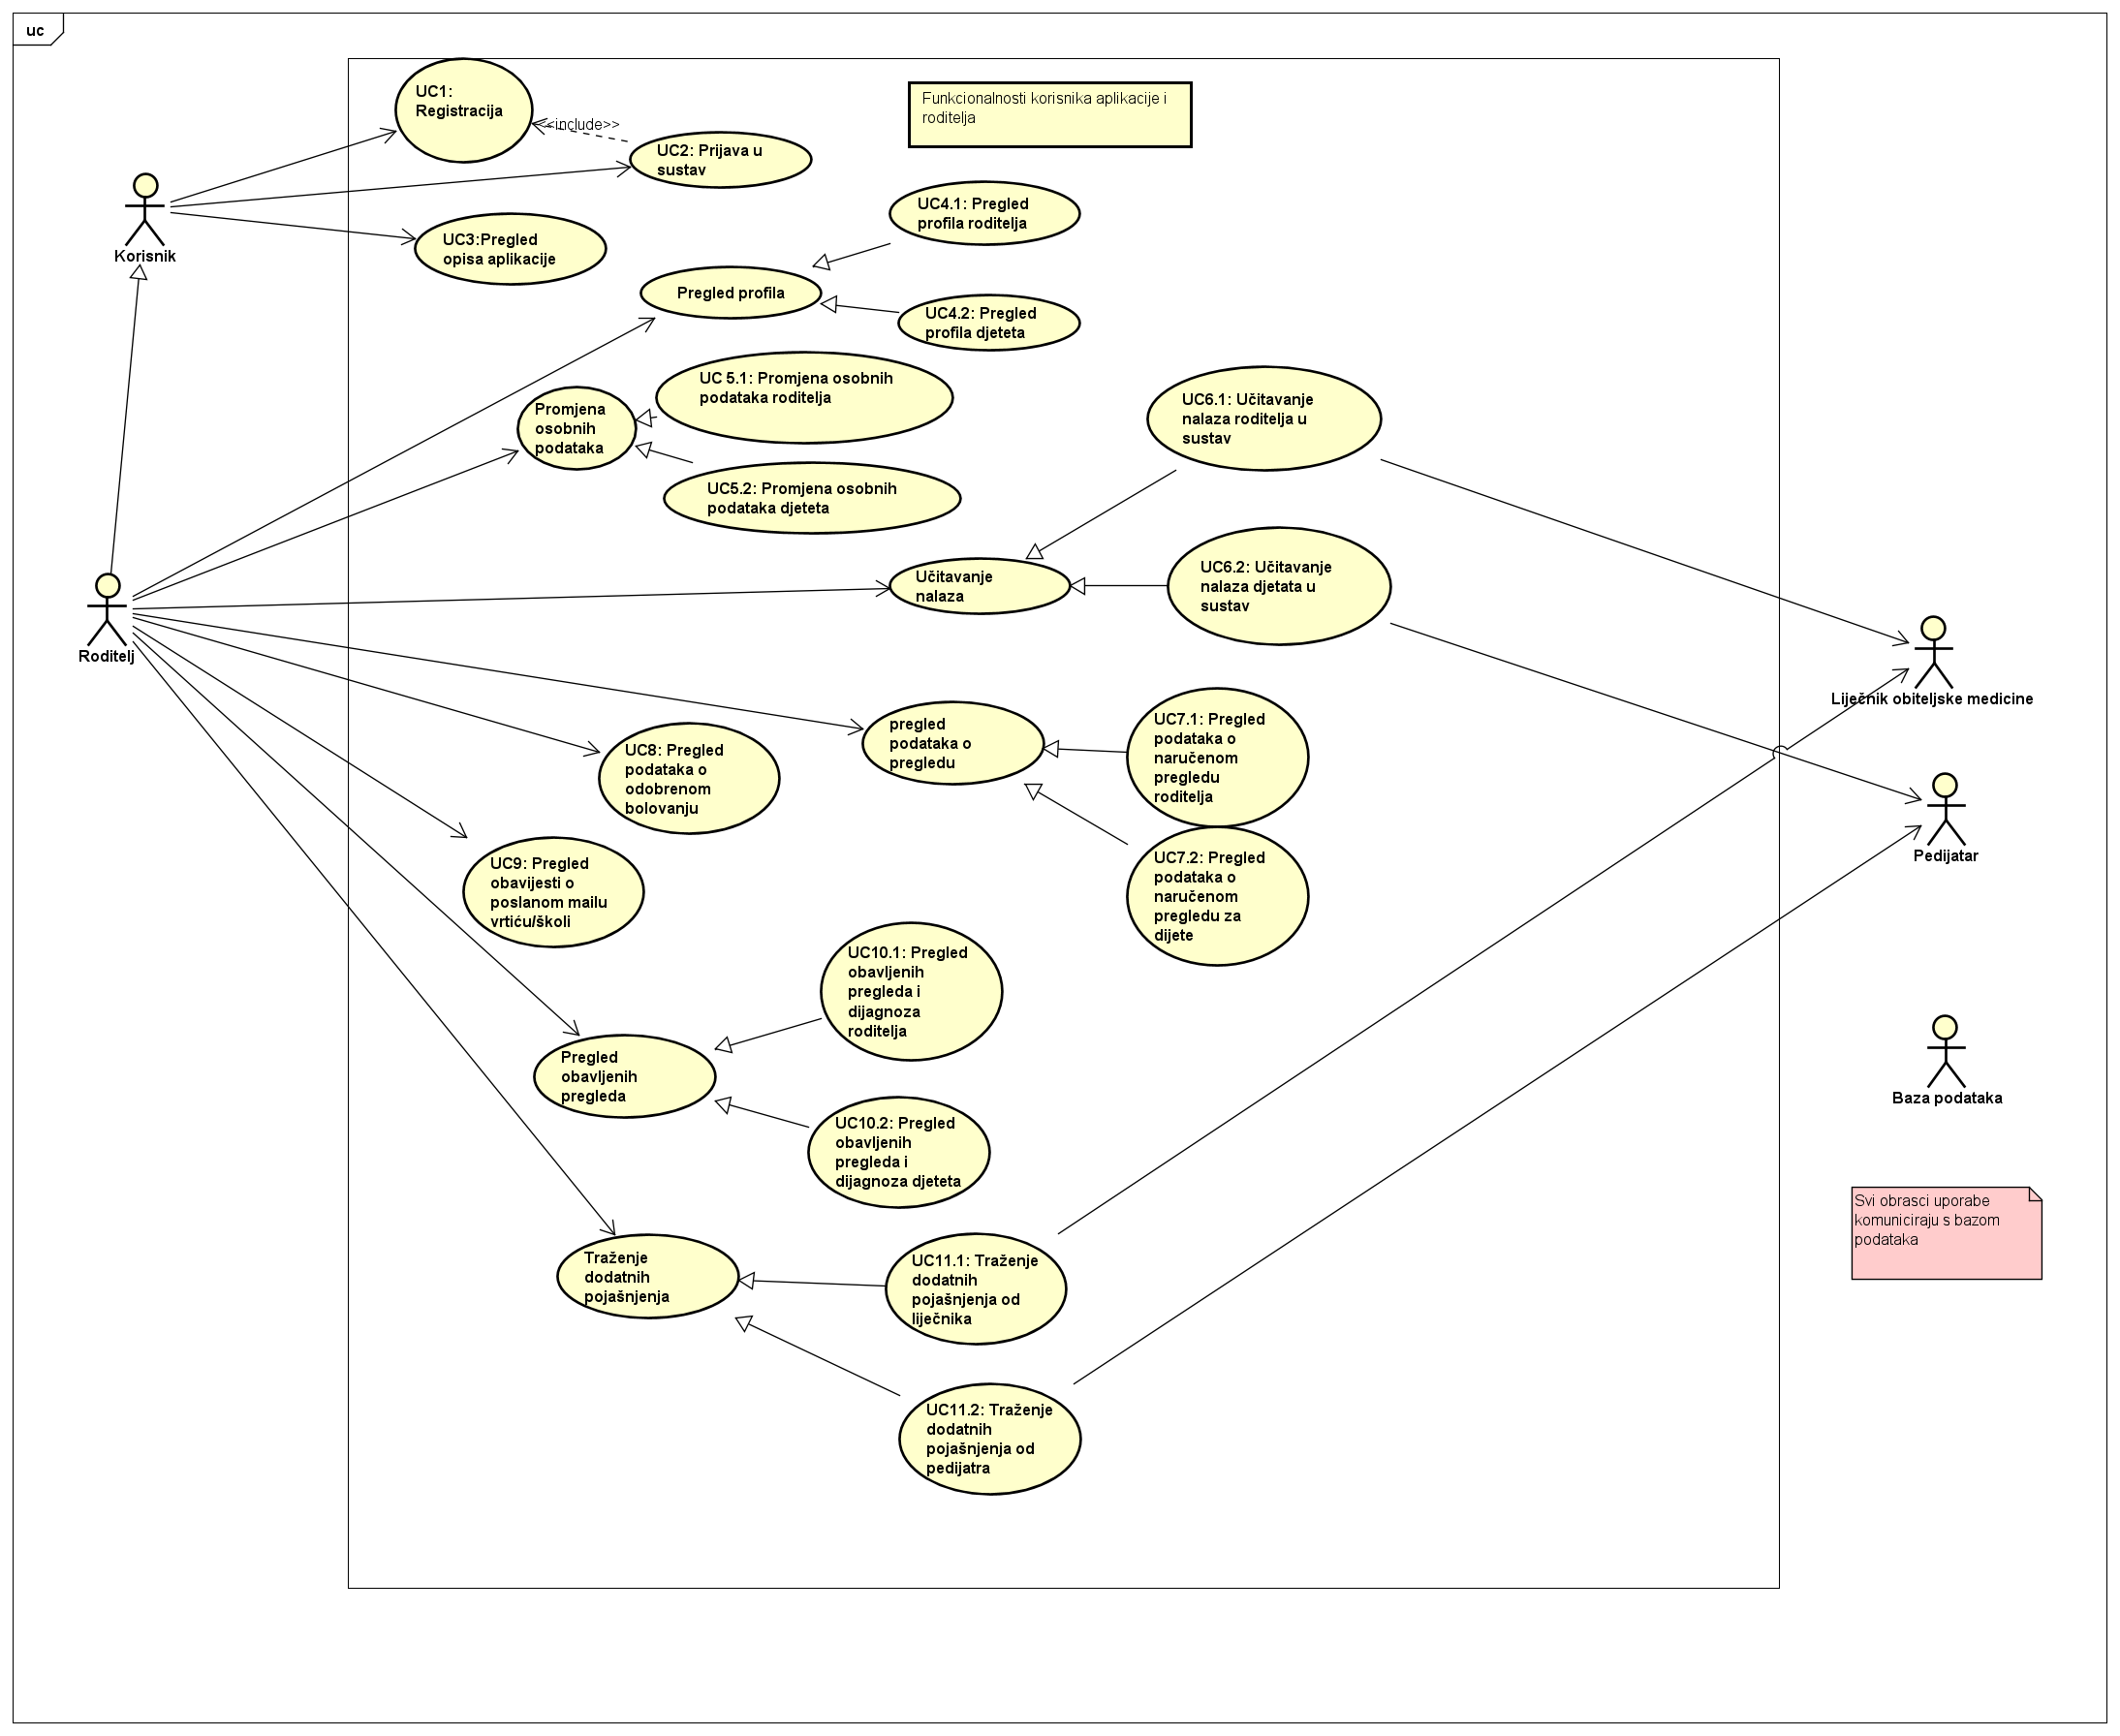
\includegraphics[width=\textwidth]{slike/UCroditelj.PNG} %veličina u odnosu na širinu linije
						\caption{UML dijagram koji opisuje obrasce uporabe korisnika i roditelja}
						\label{fig:promjene3} %label mora biti drugaciji za svaku sliku
					\end{figure}
					
					Referenciranje slike \ref{fig:promjene3} u tekstu.
					
					\begin{figure}[H]
						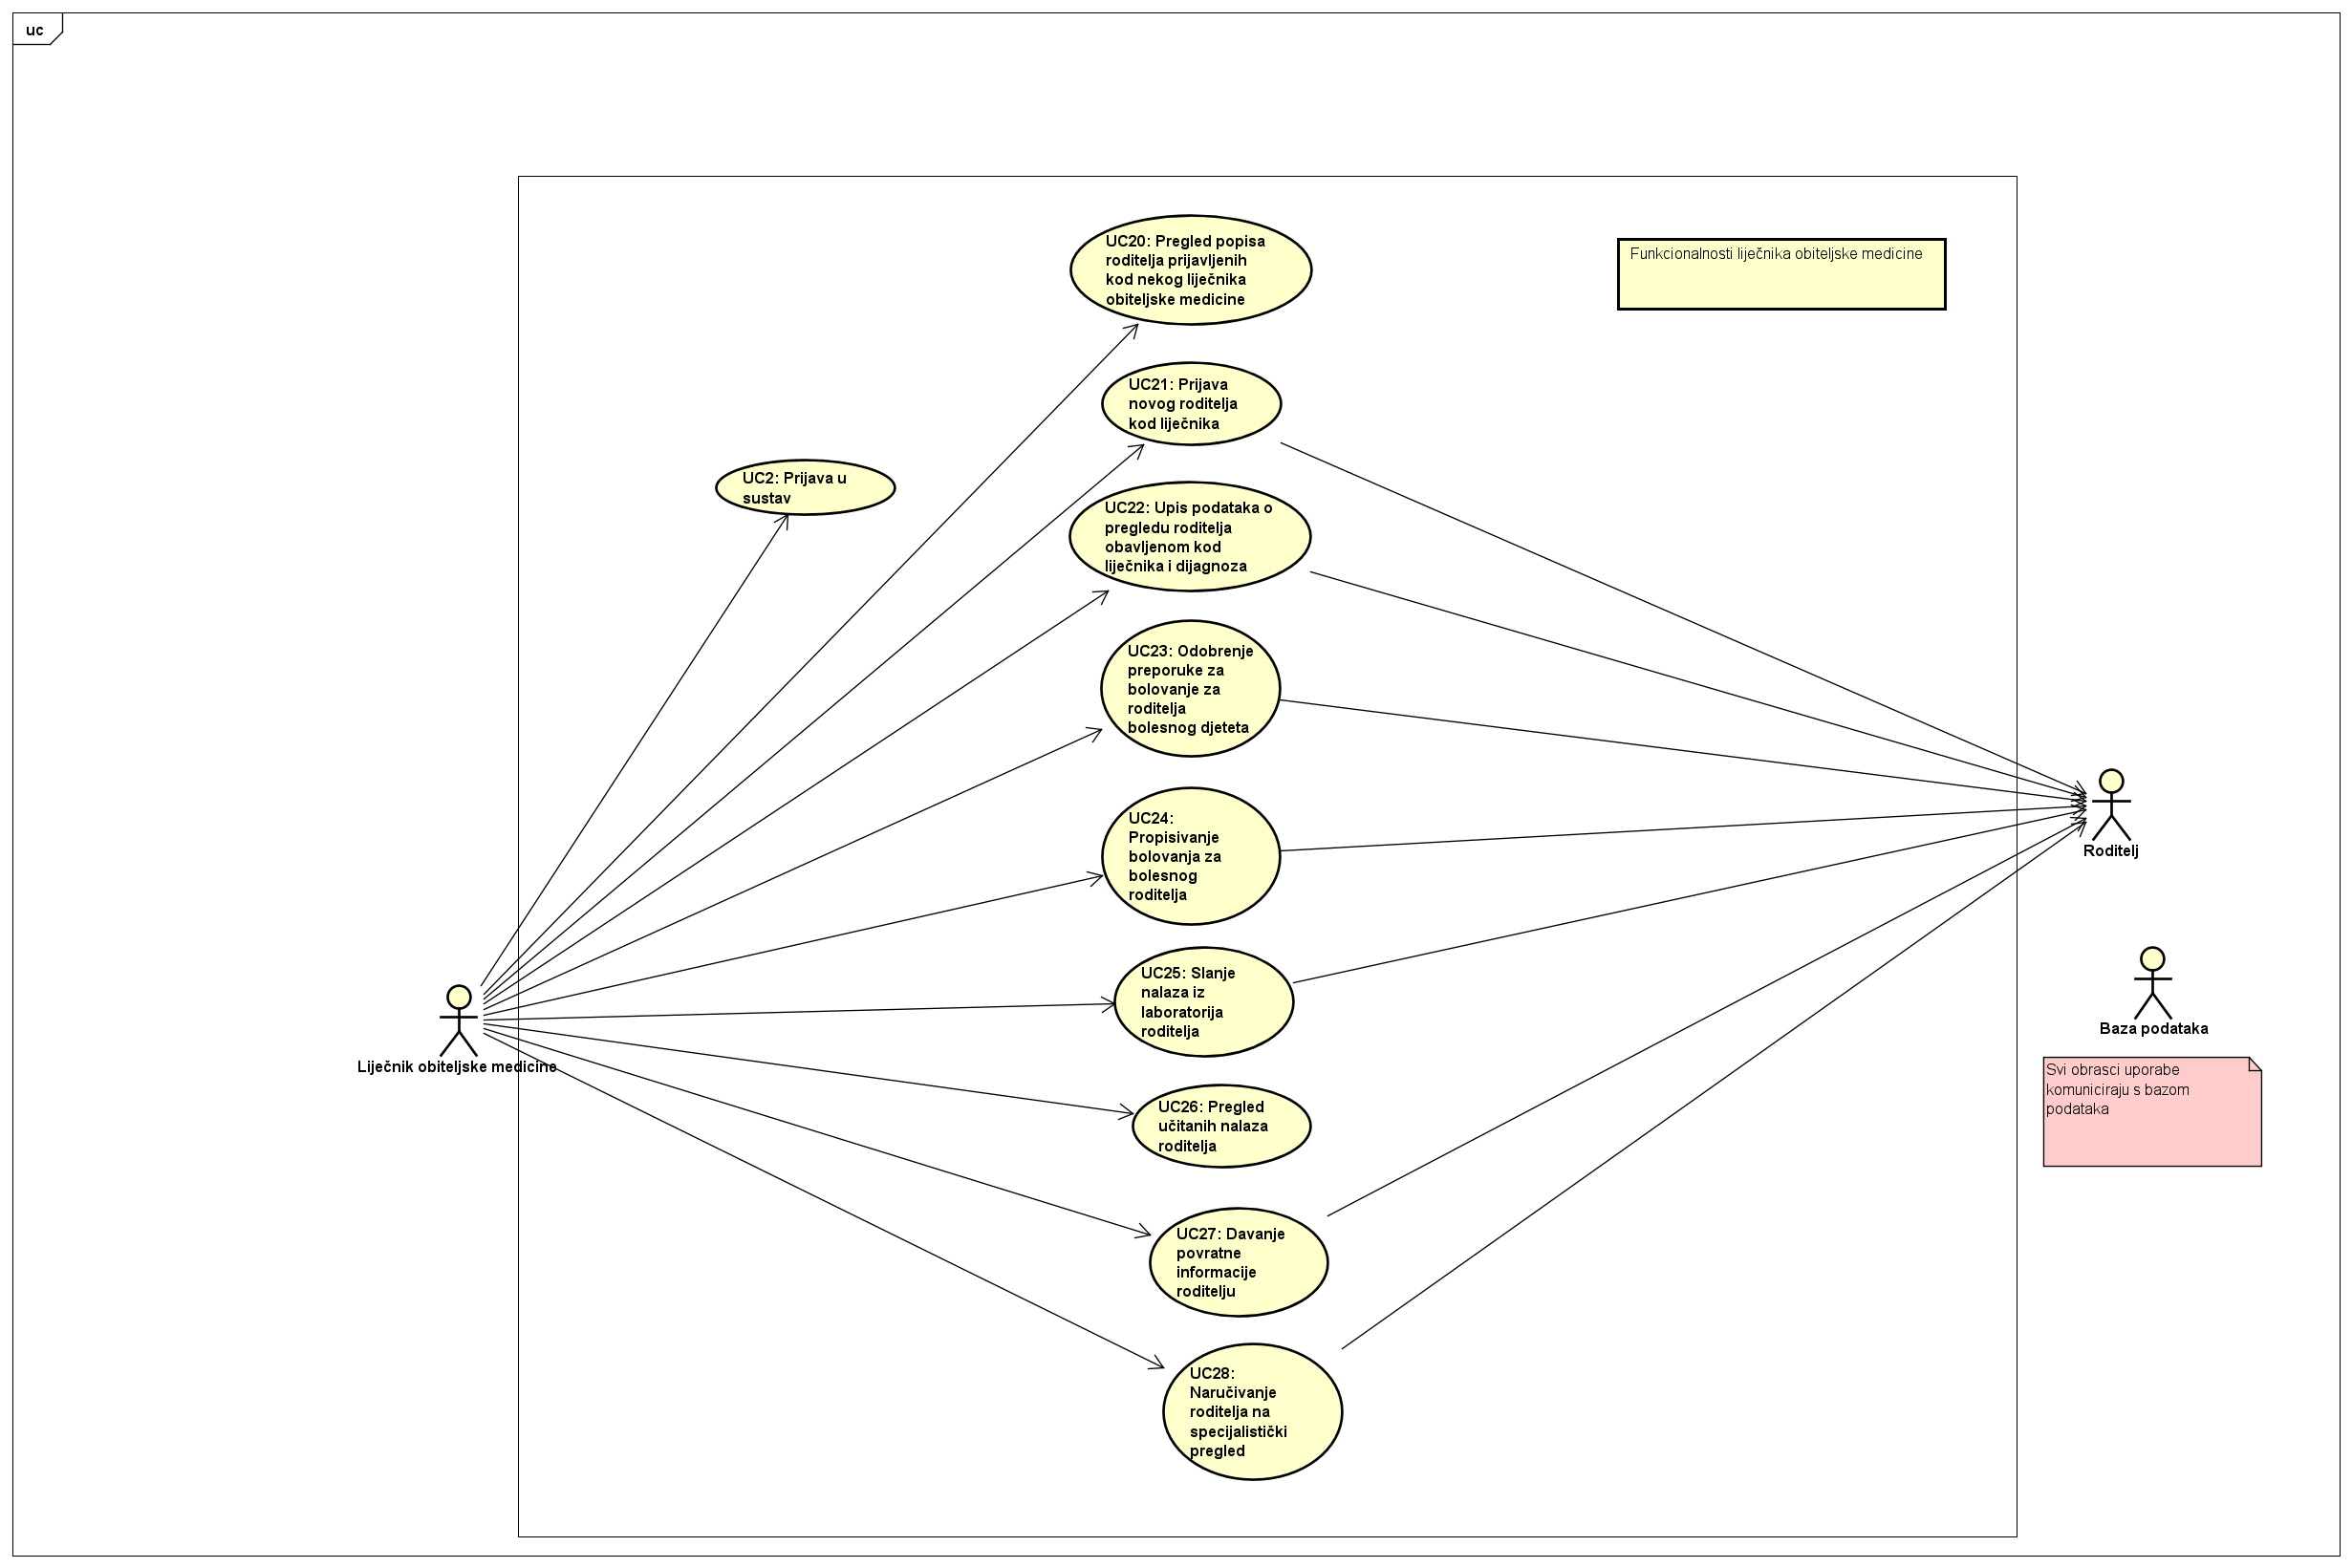
\includegraphics[width=\textwidth]{slike/UCliječnik.PNG} %veličina u odnosu na širinu linije
						\caption{UML dijagram koji opisuje obrasce uporabe liječnika}
						\label{fig:promjene4} %label mora biti drugaciji za svaku sliku
					\end{figure}
					
					Referenciranje slike \ref{fig:promjene4} u tekstu.
					
					\begin{figure}[H]
						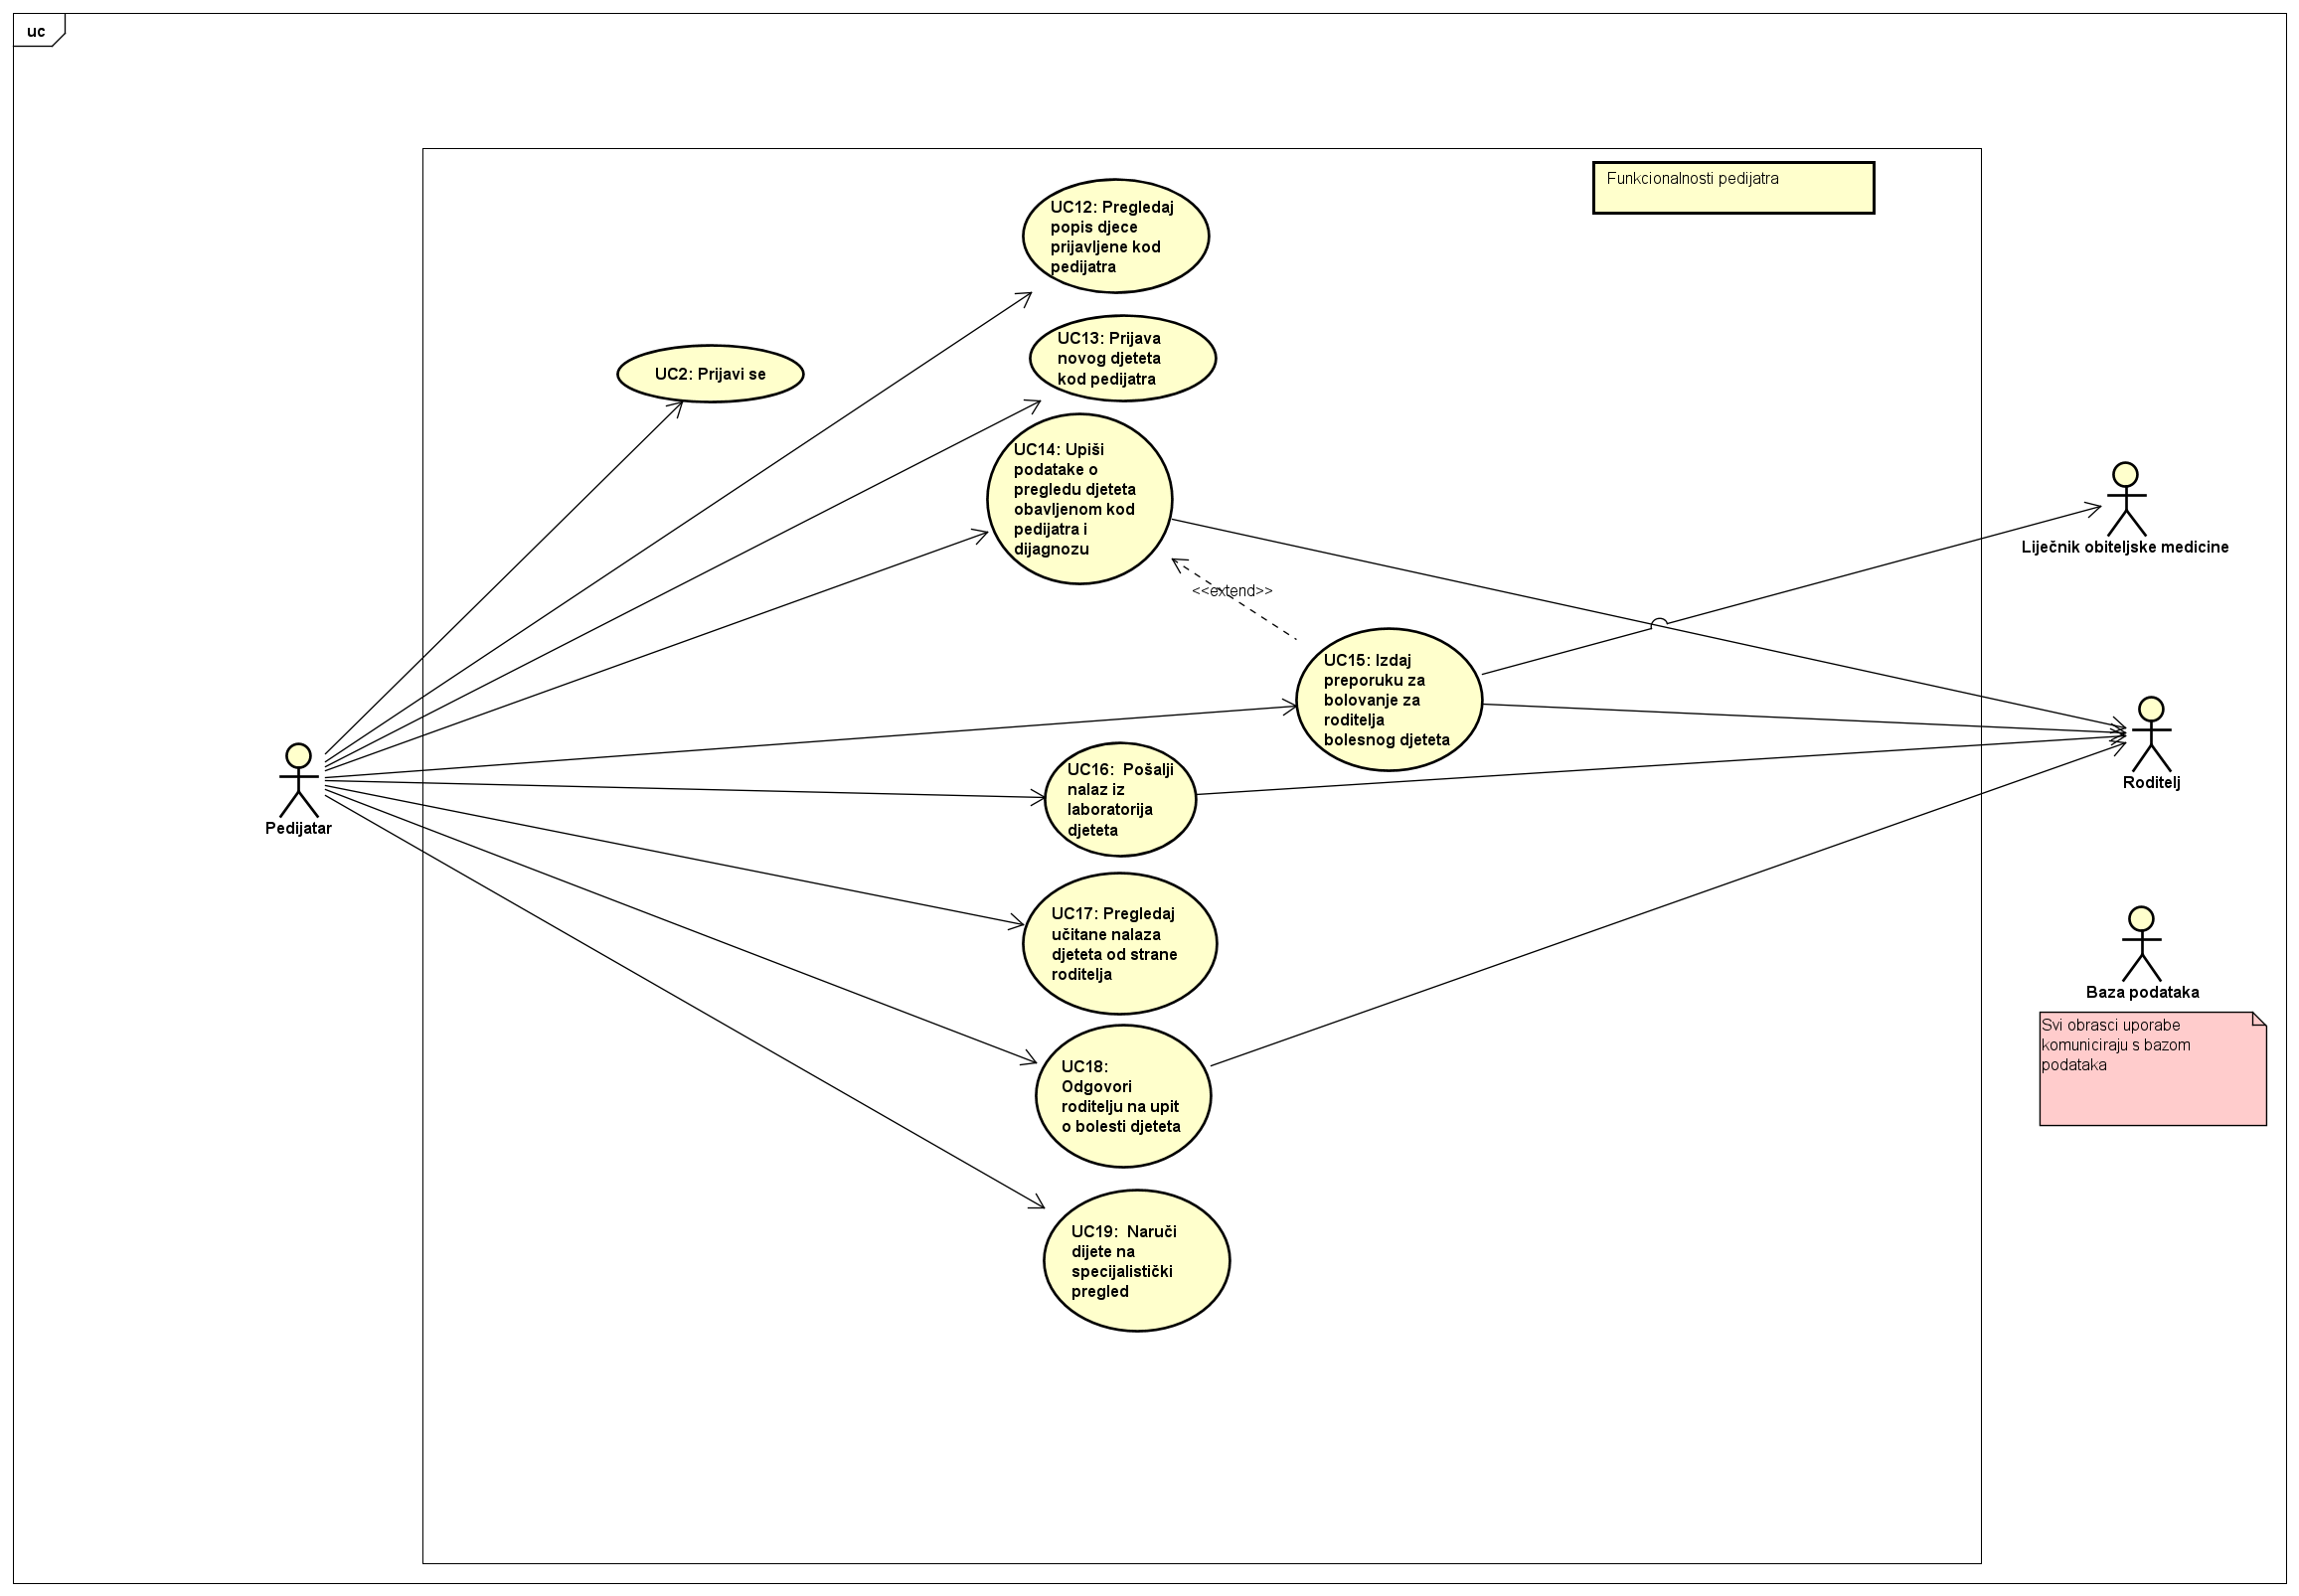
\includegraphics[width=\textwidth]{slike/UCpedijatar.PNG} %veličina u odnosu na širinu linije
						\caption{UML dijagram koji opisuje obrasce uporabe pedijatra}
						\label{fig:promjene5} %label mora biti drugaciji za svaku sliku
					\end{figure}
					
					Referenciranje slike \ref{fig:promjene5} u tekstu.
					
					\begin{figure}[H]
						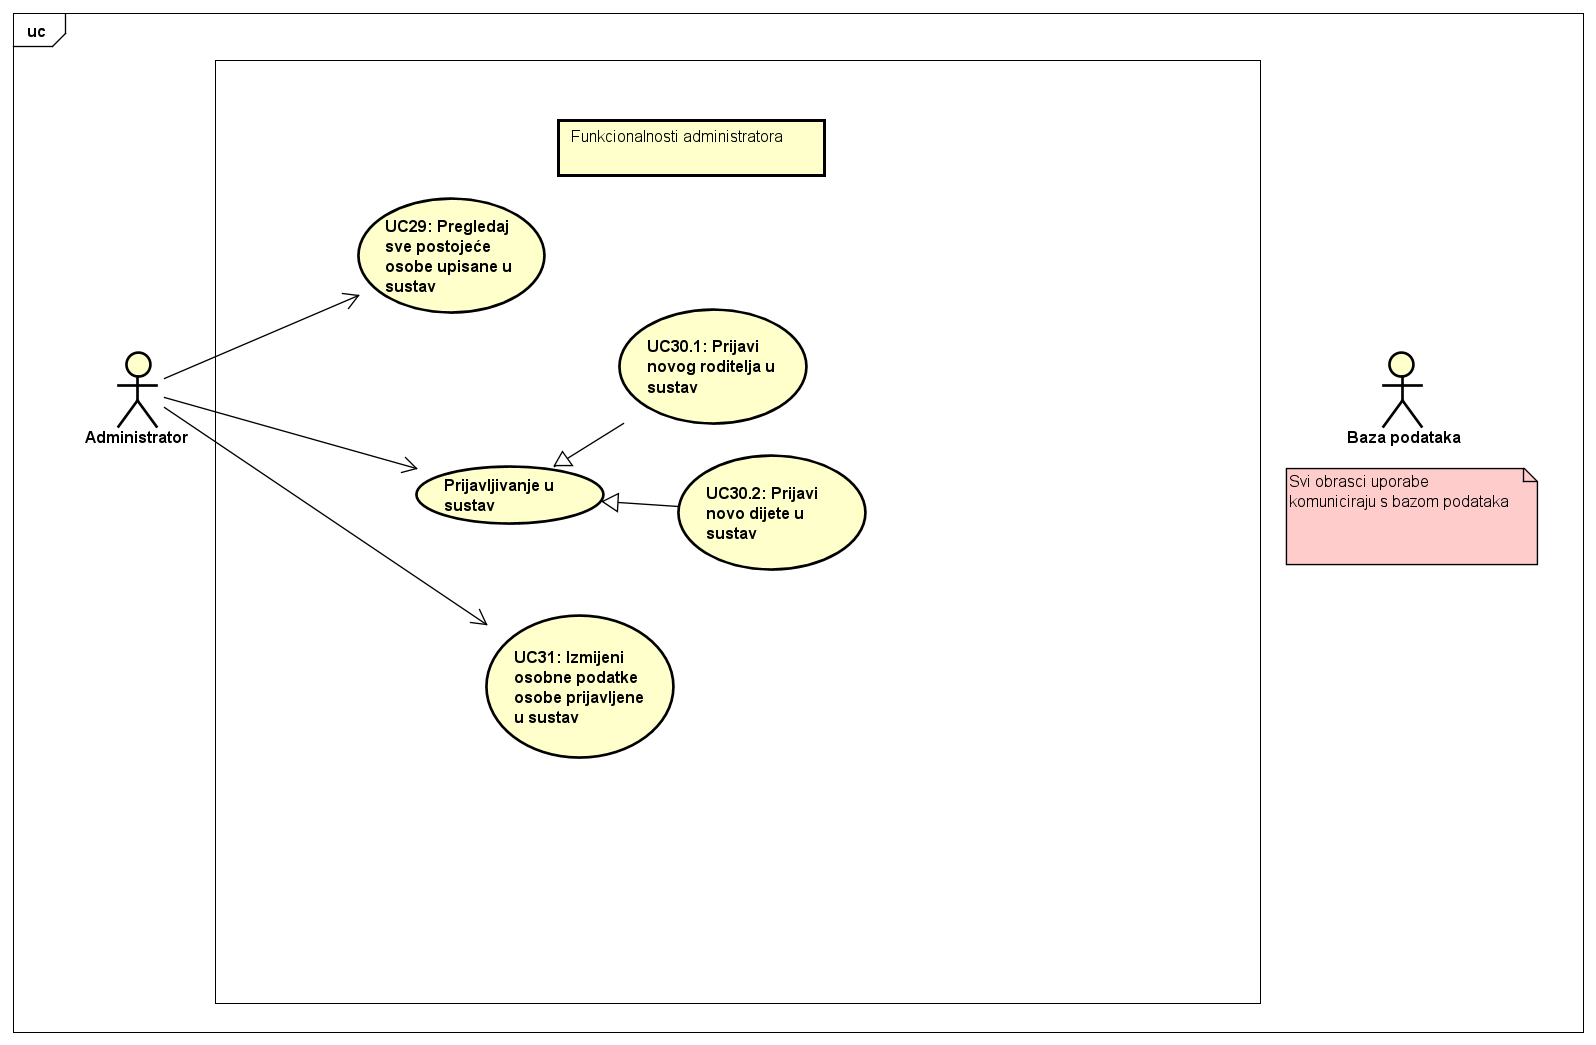
\includegraphics[width=\textwidth]{slike/UCadmin.PNG} %veličina u odnosu na širinu linije
						\caption{UML dijagram koji opisuje obrasce uporabe administratora}
						\label{fig:promjene6} %label mora biti drugaciji za svaku sliku
					\end{figure}
					
					Referenciranje slike \ref{fig:promjene6} u tekstu.
					
				
			\subsection{Sekvencijski dijagrami}
				
				\textbf{\textit{dio 1. revizije}}\\
				
					\textbf{Obrazac uporabe UC6.2 - Učitavanje nalaza djeteta u sustav, UC14 - Upis podataka o pregledu djeteta obavljenom kod pedijatra i dijagnoza, UC15 - Izdavanje preporuke za bolovanje za roditelja bolesnog djeteta, UC16 - Slanje nalaza iz laboratorija djeteta, Pregled učitanih nalaza djeteta od strane roditelja, UC23 - Odobrenje preporuke za bolovanje za roditelja bolesnog djeteta}\\
				
				
				Ulogirani roditelj učitava simptome svog bolesnog djeteta u web aplikaciju koja ga prosljeđuje pedijatru koji dijete naručuje na pregled te nakon pregleda roditelju šalje laboratorijski nalaz te po mogućnosti šalje ispričnicu za školu/vrtić roditelju te preporuku za bolovanje liječniku. Ako liječnik odobri bolovanje roditelju, preko aplikacije mu pošalje potvrdu.
				
				\begin{figure}[H]
					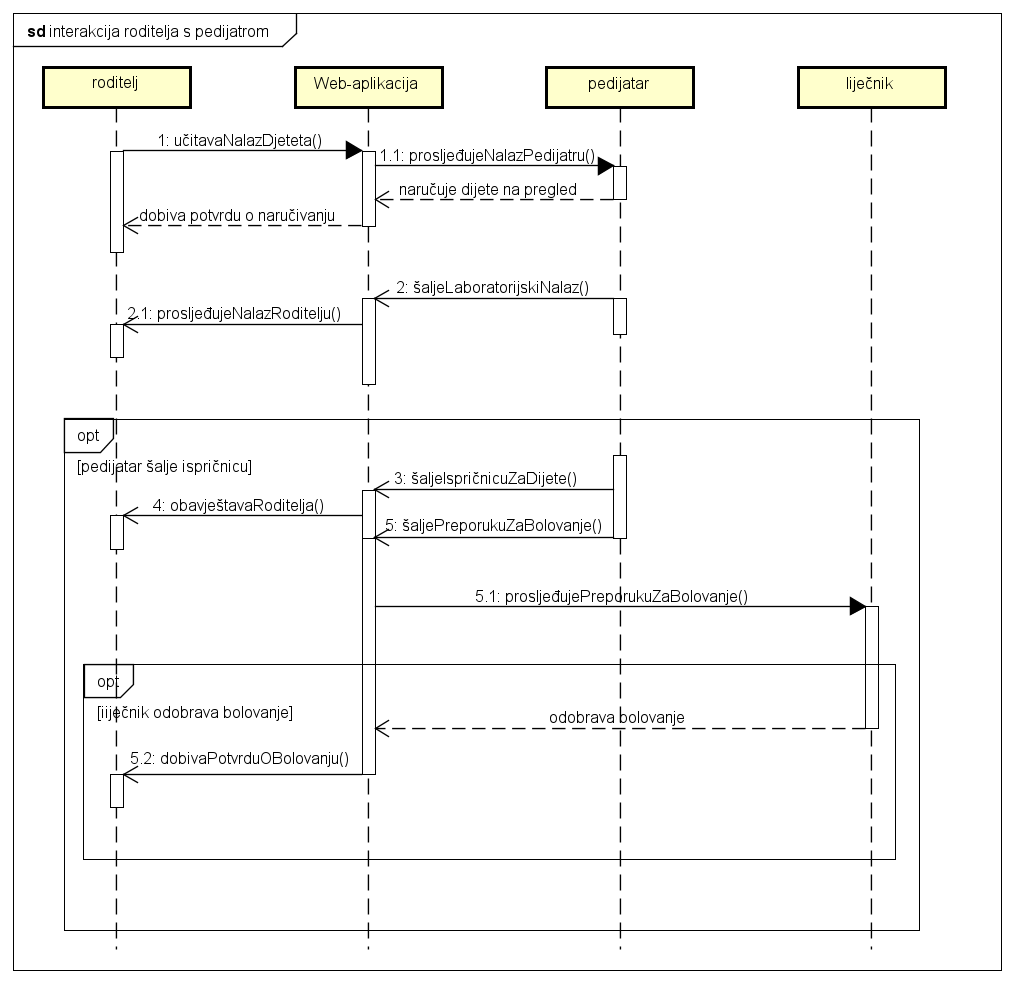
\includegraphics[width=\textwidth]{slike/SDrplW.PNG} %veličina u odnosu na širinu linije
					\caption{Sekvencijski dijagram koji opisuje osnovnu mehaniku naručivanja djeteta i roditelja na pregled}
					\label{fig:promjene7} %label mora biti drugaciji za svaku sliku
				\end{figure}
				
				
				\textbf{Obrazac uporabe UC30.1 - Prijavljivanje novog roditelja u sustav, UC30.2 - Prijavljivanje novog djeteta u sustav}\\
				
				Administrator se ulogirava u sustav i na početnoj stranici bira opciju dodaj roditelja te upisuje njegovo ime, prezime, OIB i datum rođenja. Pritiskom na opciju dodaj u bazu podataka se taj roditelj dodaje. Potom Administrator pokuša upisati novo dijete upisom njegovog imena, prezimena OIB-a, datuma rođenja djeteta te iz liste koja mu se aplikaciji proslijedi iz baze podataka odabere OIB roditelja djeteta kojeg želi upisati u sustav. Potom odabere opciju Dodaj te se baza podataka obnovi.
				\eject
				
				\begin{figure}[H]
					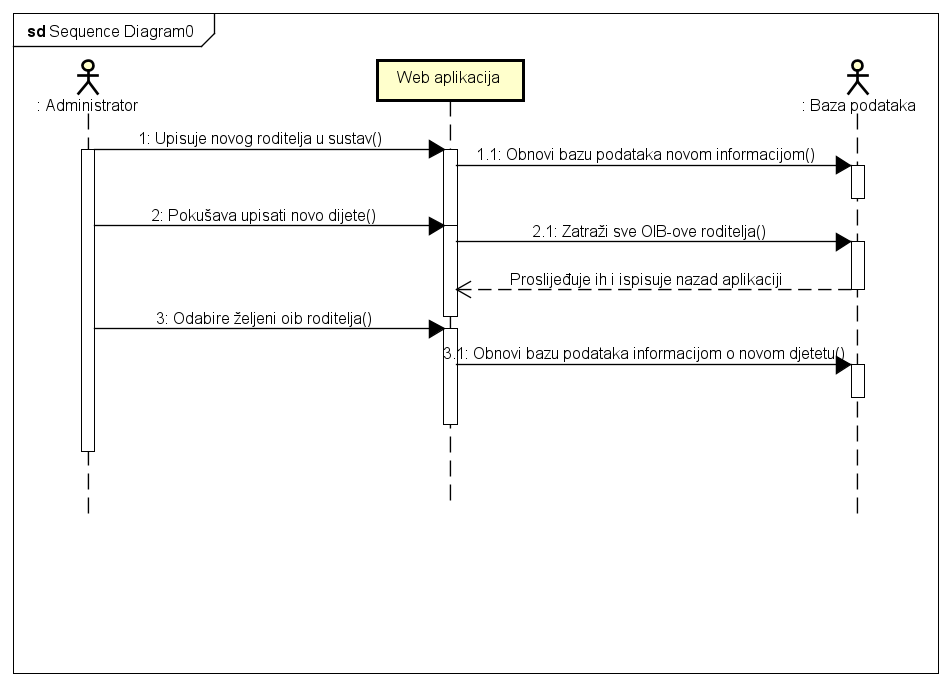
\includegraphics[width=\textwidth]{slike/SDadminapp.PNG} %veličina u odnosu na širinu linije
					\caption{Sekvencijski dijagram za UC30.1 i UC30.2}
					\label{fig:promjene8} %label mora biti drugaciji za svaku sliku
				\end{figure}
				
				
				
				\textbf{Obrazac uporabe UC5.1 - Promjena osobnih podataka roditelja, UC5.2 - Promjena osobnih podataka djeteta}\\
			
				
				Klijent se ulogirava u sustav unosom OIB-a i korisničke lozinke. Nakon provjere postoji li korisnički profil s danim podatcima u bazi, popis dostupnih profila se dohvaća iz baze i ispisuje korisniku. Korisnik odabire profil (vlastiti ili djetetov) te poslužitelj dohvaća podatke iz baze i ispisuje korisnički profil. Odabirom opcije "Pregled osobnih podataka" poslužitelj će iz baze dohvatiti osobne podatke korisnika te ih ispisati na ekran. Korisnik potom uređuje podatke te odabirom opcije "spremi" promjene pohranjuje u bazu. Preglednik će zatim dohvatiti početnu stranicu profila i prikazati ju korisniku.
				\eject
				
				\begin{figure}[H]
					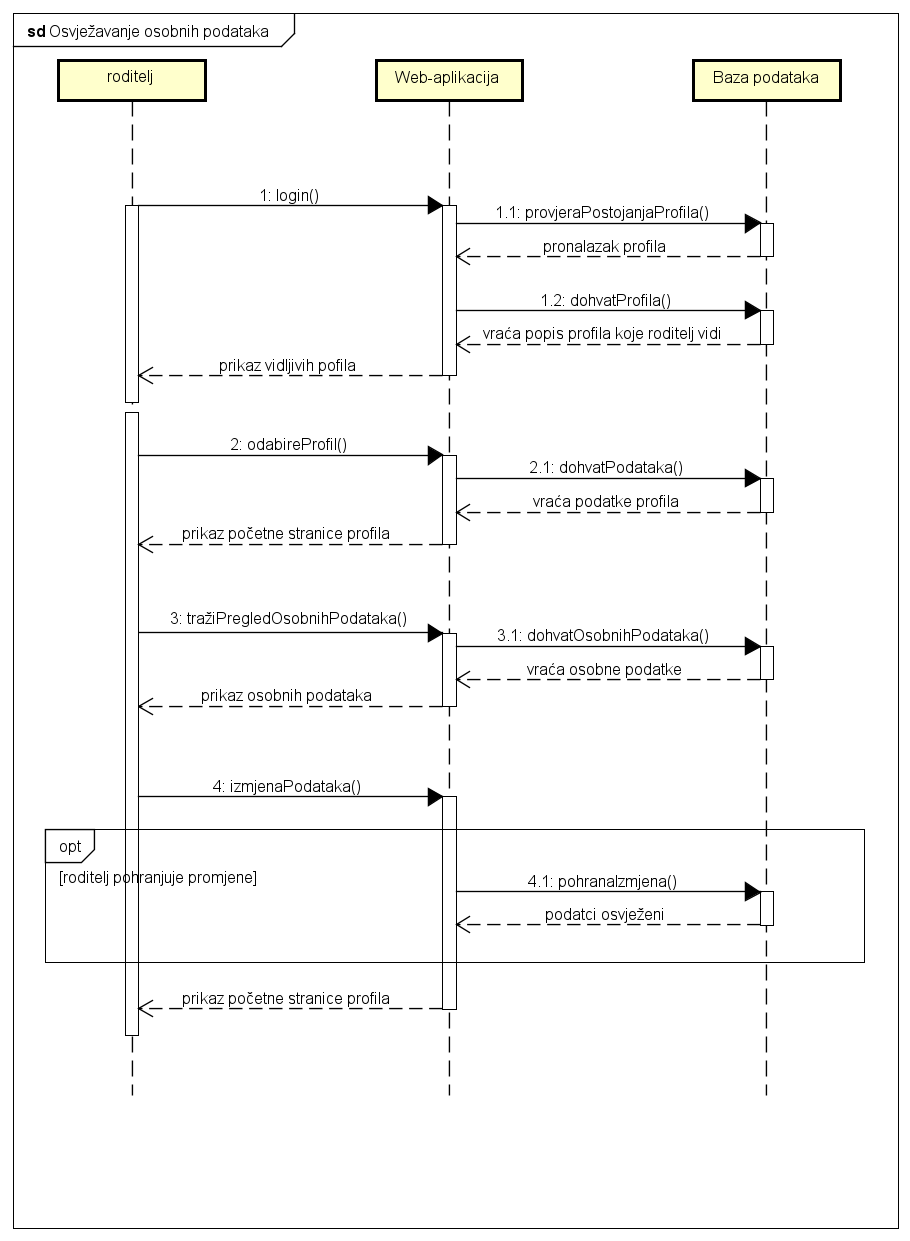
\includegraphics[scale=0.6]{dijagrami/OsobniPodatci.PNG} %veličina slike u odnosu na originalnu datoteku i pozicija slike
					\centering
					\caption{Sekvencijski dijagram za UC5.1 i UC5.2}
					\label{fig:sekvencijski1}
				\end{figure}
				
				\eject
				
				
				
					\textbf{Obrazac uporabe UC13 - Prijava novog djeteta kod pedijatra, UC21 - Prijava novog roditelja kod liječnika}\\
				
				
				Liječnik (pedijatar) se ulogirava u sustav unosom OIB-a i korisničke lozinke. Preglednik poziva bazu i provjerava postoji li korisnički profil u bazi nakon čega iz baze dohvaća upisane pacijente dotičnog korisnika te ih ispisuje na ekran. Korisnik odabire opciju "Prijavi novo(g) dijete/roditelja". Preglednik iz baze dohvaća popis neupisanih pacijenata te ih ispisuje na ekran. Odabirom pacijenta preglednik u bazu upisuje novog pacijenta liječniku/pedijatru, dohvaća osvježenu tablicu upisanih pacijenata te korisniku ispisuje početnu stranicu s upisanim pacijentima.
				
				
				\begin{figure}[H]
					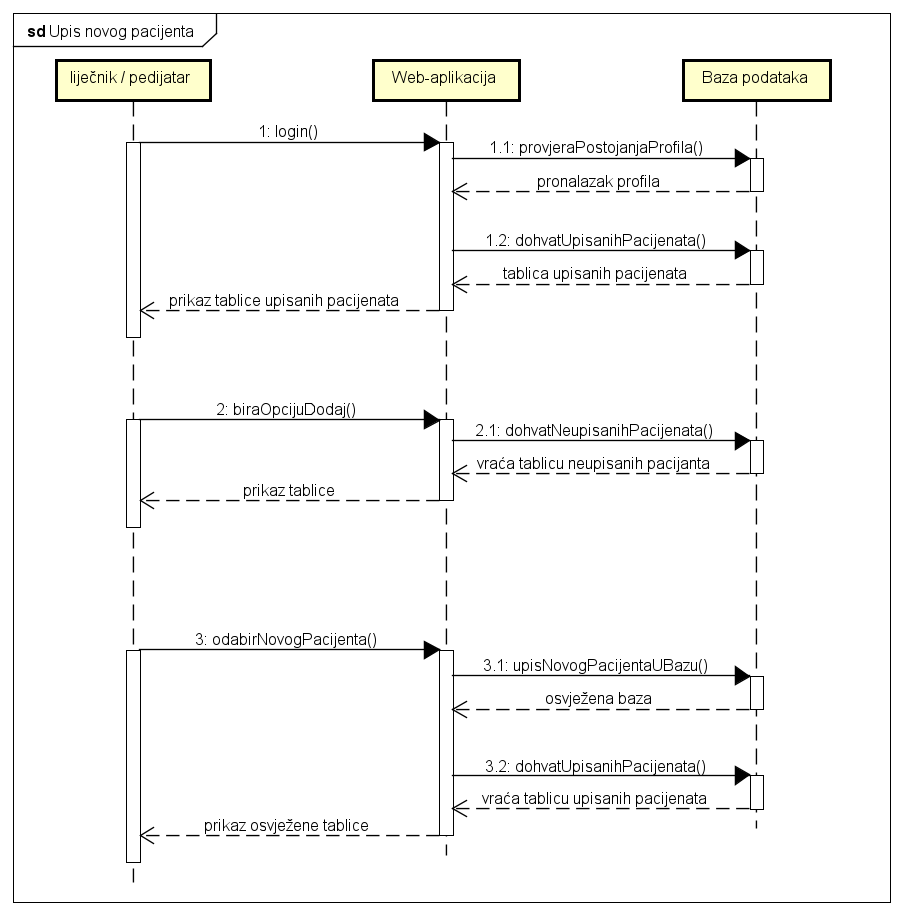
\includegraphics[scale=0.6]{dijagrami/UpisNovogPacijenta.PNG} %veličina slike u odnosu na originalnu datoteku i pozicija slike
					\centering
					\caption{Sekvencijski dijagram za UC13 i UC21}
					\label{fig:sekvencijski2}
				\end{figure}
				
				\eject
	
		\section{Ostali zahtjevi}
		
			\textbf{\textit{dio 1. revizije}}\\
		 
			 \textit{Nefunkcionalni zahtjevi i zahtjevi domene primjene dopunjuju funkcionalne zahtjeve. Oni opisuju \textbf{kako se sustav treba ponašati} i koja \textbf{ograničenja} treba poštivati (performanse, korisničko iskustvo, pouzdanost, standardi kvalitete, sigurnost...). Primjeri takvih zahtjeva u Vašem projektu mogu biti: podržani jezici korisničkog sučelja, vrijeme odziva, najveći mogući podržani broj korisnika, podržane web/mobilne platforme, razina zaštite (protokoli komunikacije, kriptiranje...)... Svaki takav zahtjev potrebno je navesti u jednoj ili dvije rečenice.}
			 
			 
			 
	
	\chapter{Arhitektura i dizajn sustava}
		
		Arhitektura se može podijeliti na nekoliko podsustava:
		 \begin{itemize}
			\item Poslužitelj frontenda
			\item Frontend (prvi dio web aplikacije)
			\item Poslužitelj backenda
			\item Backend (drugi dio web aplikacije)
			\item Baza podataka 
		\end{itemize}
		
		\begin{figure}[H]
			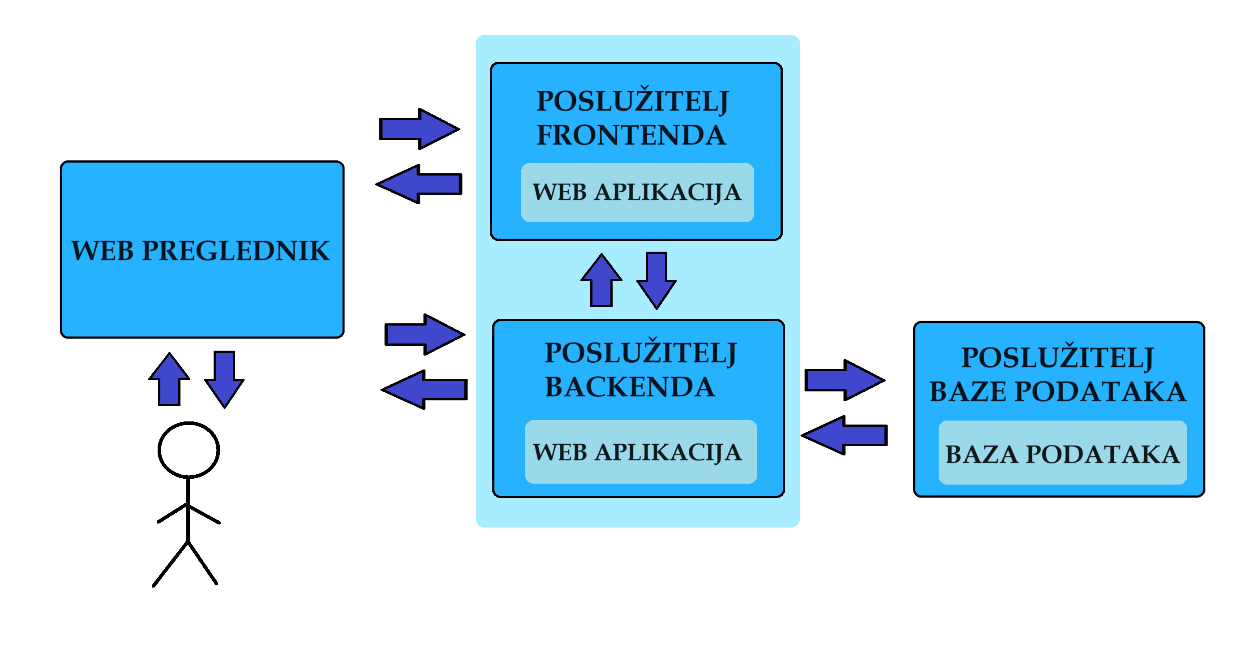
\includegraphics[width=\textwidth]{slike/arhitekturaSustava.PNG} %veličina u odnosu na širinu linije
			\caption{Arhitektura sustava}
			\label{fig:promjene9} %label mora biti drugaciji za svaku sliku
		\end{figure}
		
		 \underbar{\textit{Web preglednik}} je program koji omogućuje korisnicima pregled web sadržaja, a to uključuje web stranice i njihov raznolik sadržaj (slike, dijagrami...). Web preglednik je i okolina u kojoj se mogu izvršiti skripte (potrebno npr. kod client-side renderinga). Jedna od glavnih funkcionalnosti web preglednika je slanje zahtjeva prema web poslužiteljima.
		 	
		 \underbar{\textit{Frontend poslužitelj}} je poslužitelj koji komunicira s web preglednikom klijenta preko HTTP (\textit{engl. Hyper Text Transfer Protocol}) protokola. Na frontend poslužitelju se nalazi frontend dio web aplikacije čije dijelove frontend poslužitelj vraća klijentu na zahtjev (npr. pri početnom otvaranju stranice).
		 
		 \underbar{\textit{Backend poslužitelj}} je poslužitelj na kojem se nalazi backend dio aplikacije. Backend poslužitelj omogućuje slanje i primanje zahtjeva backend dijelu aplikacije. Backend poslužitelj preko HTTP protokola komunicira s frontendom ili web preglednikom klijenta. Ovaj poslužitelj komunicira i s poslužiteljem baze podataka preko TCP (eng. Transmission Control Protocol) protokola.
		 
		 \underbar{\textit{Web aplikacija}} dijeli se na frontend i backend. Zadaća frontend dijela je oblikovanje prikaza podataka, a potrebne podatke može zatražiti od backenda. Zadaća backend dijela je dohvaćanje podataka iz baze te njihova obrada i prosljeđivanje frontendu u određenom obliku. Komunikacija između frontenda, backenda, baze i web preglednika odvija se preko zahtjeva.
		 
		 \underbar{\textit{Baza podataka}} sadrži sve informacije o korisničkim računima, korisnicima te porukama koje korisnici šalju unutar web aplikacije.\\
		 	
		 Razvojni okvir koji smo odabrali za razvijanje backend dijela aplikacije jest Spring (programski jezik Java). Za razvoj frontend dijela aplikacije odlučili smo se za razvojni okvir React (programski jezik JavaScript). Odabrano razvojno okruženje je IntelliJ IDEA. Baza podataka napravljena je koristeći PostgreSQL.\\
		 
		 Arhitektura web aplikacije temelji se na single-page application principu kojeg omogućuje razvojni okvir React. Pri početnom otvaranju web aplikacije, web preglednik korisnika uputi zahtjev frontend serveru koji mu vraća sve odgovarajuće datoteke potrebne za prikaz stranice u pregledniku (koristi se princip client-side rendering). Ovisno o prosljeđenim podacima, web preglednik prilikom obrađivanja ulaznih podataka korisnika (klik na pojedini gumb, otvaranje nove stranice) šalje zahtjeve backend serveru (ako su potrebni određeni podaci za prikaz React komponente) ili frontend serveru (za dohvat datoteka potrebnih za prikaz novog dijela stranice).
		 
		  	
		  

	
		

		

				
		\section{Baza podataka}
			
		
		Za našu web aplikaciju koristiti ćemo relacijsku bazu podataka koja je industrijski standard te najjednostavniji način za rješenje našeg problema. Osnovni element baze je relacija čija su obilježja njeno ime i atributi. Glavna zadaća naše baze je spajanje njenih korisnika i sustava s korisnikom, bilo kroz poruke ili kroz razne obrasce. Postoji jedna tablica veza s nazivom Pregled.
		Entiteti ove baze podataka su:
		
			\begin{packed_item}
				\item Osoba
				\item Poruka
				\item Bolest
				\item Bolnica
			\end{packed_item}
		
		
			\subsection{Opis tablica}
				
				
				\textbf{Osoba} Ovaj entitet sadrži sve informacije o pojedinoj osobi spremljenoj u aplikaciji. Budući da ovaj entitet modelira i građane i zdravstvene zaposlenike ima mnogo opcionalnih atributa. Atributi entiteta su: OIB, ime, prezime,lozinka, email ustanove, datum rođenja, adresa stanovanja, administratorska prava,uloga, OIB roditelja i OIB zadanog doktora. Moguće uloge su: 'roditelj','dijete','pedijatar','doktor'. Email ustanove, datum rođenja, adresa stanovanja, lozinka, OIB roditelja i OIB doktora mogu biti prazni. Ovaj entitet je u \textit{Many-to-One} vezi s entitetom Osoba s ulogom roditelj preko atributa rodOIB,\textit{Many-to-One} vezi s entitetom Osoba s ulogom liječnik preko dokOIB, \textit{One-to-Many} vezi s Poruka preko OIB-a gdje jedan entitet Poruka zahtjeva dva entiteta Osoba.
				
				\begin{longtblr}[
					label=none,
					entry=none
					]{
						width = \textwidth,
						colspec={|X[6,l]|X[6, l]|X[20, l]|}, 
						rowhead = 1,
					} %definicija širine tablice, širine stupaca, poravnanje i broja redaka naslova tablice
					\hline \SetCell[c=3]{c}{\textbf{Osoba}}	 \\ \hline[3pt]
					\SetCell{LightGreen}OIB & INT	&  	OIB osobe  	\\ \hline
					ime	& VARCHAR & ime osobe   	\\ \hline 
					prezime & VARCHAR & prezime osobe   \\ \hline 
					mail & VARCHAR	& email ustanove (opcionalno)  \\ \hline
					datumRod & DATETIME & datum rođenja osobe (opcionalno)  \\ \hline
					adresa & VARCHAR & adresa stanovanja (opcionalno)   \\ \hline    
					adminPrava & INT & administratorska prava (0 ili 1)   \\ \hline
					lozinka	& VARCHAR & šifra računa osobe (opcionalno)	\\ \hline
					uloga	& VARCHAR & uloga osobe	\\ \hline
					\SetCell{LightBlue} rodOIB	& INT & OIB roditelja	\\ \hline
					\SetCell{LightBlue} dokOIB	& INT & OIB doktora  	\\ \hline 
				\end{longtblr}
				
				
				
				\textbf{Poruka} Ovaj entitet sadrži sve informacije o porukama spremljenima u aplikaciji. Njegovi atributi su: id, OIBpoš, OIBpri, naslov, tijelo, prilog, tip, dijagnoza. Prilog i dijagnoza mogu biti prazne, ovisno o tipu poruke. Ovaj entitet je u \textit{Many-to-One} vezi s entitetom Osoba preko OIB-a te su potrebna 2 različita OIB-a,\textit{Many-to-One} vezi s entitetom Bolest preko id-a.
				
				\begin{longtblr}[
					label=none,
					entry=none
					]{
						width = \textwidth,
						colspec={|X[6,l]|X[6, l]|X[20, l]|}, 
						rowhead = 1,
					} %definicija širine tablice, širine stupaca, poravnanje i broja redaka naslova tablice
					\hline \SetCell[c=3]{c}{\textbf{Poruka}}	 \\ \hline[3pt]
					\SetCell{LightGreen}id & INT	&  	identifikacijski ključ poruke	\\ \hline
					\SetCell{LightBlue} priOIB	& INT & OIB pošiljatelja	\\ \hline
					\SetCell{LightBlue} pošOIB	& INT & OIB primatelja	\\ \hline
					naslov	& VARCHAR & naslov poruke  	\\ \hline
					tijelo	& VARCHAR & tekstualni sadržaj poruke  	\\ \hline
					prilog	& VARCHAR & link na poslanu sliku unutar datotečnog sustava aplikacije (opcionalno)	\\ \hline
					tip	& VARCHAR & tip poslane poruke (standardna,ispričnica itd.)	\\ \hline
					\SetCell{LightBlue}dijagnozaID	& INT & id dijagnosticirane bolesti (opcionalno)	\\ \hline      
				\end{longtblr}
				
				\textbf{Bolest} Ovaj entitet sadrži sve informacije o bolestima spremljenima u aplikaciji. Njegovi atributi su: id i naziv. Ovaj entitet je u \textit{Many-to-Many} vezama s entitetom Bolnica id-a bolnice,\textit{One-to-One} vezi s entitetom Poruka preko id-a bolesti.
				
				\begin{longtblr}[
					label=none,
					entry=none
					]{
						width = \textwidth,
						colspec={|X[6,l]|X[6, l]|X[20, l]|}, 
						rowhead = 1,
					} %definicija širine tablice, širine stupaca, poravnanje i broja redaka naslova tablice
					\hline \SetCell[c=3]{c}{\textbf{Bolest}}	 \\ \hline[3pt]
					\SetCell{LightGreen}idBolest & INT	&  	identifikacijski ključ bolesti	\\ \hline
					naziv	& VARCHAR & naziv bolesti	\\ \hline   
				\end{longtblr}
				
				\textbf{Bolnica} Ovaj entitet sadrži sve informacije o bolnici spremljenima u aplikaciji. Njegovi atributi su: id,naziv i adresa. Ovaj entitet je u \textit{Many-to-Many} vezama s entitetom Bolest preko id-a bolesti.
				
				\begin{longtblr}[
					label=none,
					entry=none
					]{
						width = \textwidth,
						colspec={|X[6,l]|X[6, l]|X[20, l]|}, 
						rowhead = 1,
					} %definicija širine tablice, širine stupaca, poravnanje i broja redaka naslova tablice
					\hline \SetCell[c=3]{c}{\textbf{Bolnica}}	 \\ \hline[3pt]
					\SetCell{LightGreen}idBolnica & INT	&  	identifikacijski ključ bolnice	\\ \hline
					naziv	& VARCHAR & naziv bolnice	\\ \hline
					adresa	& VARCHAR & adresa bolnice	\\ \hline    
				\end{longtblr}
				
				\textbf{Pregled} Ova tablica sadrži sve veze između entiteta Bolest i Bolnica spremljene u aplikaciji koji su u \textit{Many-to-Many} vezi. Atributi teblice su: idBolest i idBolnica. 
				
				\begin{longtblr}[
					label=none,
					entry=none
					]{
						width = \textwidth,
						colspec={|X[6,l]|X[6, l]|X[20, l]|}, 
						rowhead = 1,
					} %definicija širine tablice, širine stupaca, poravnanje i broja redaka naslova tablice
					\hline \SetCell[c=3]{c}{\textbf{Pregled}}	 \\ \hline[3pt]
					\SetCell{LightBlue}idBolest & INT	&  	identifikacijski ključ bolesti	\\ \hline
					\SetCell{LightBlue}idBolnica	& INT & identifikacijski ključ bolnice  \\ \hline
				\end{longtblr}
			
			\subsection{Dijagram baze podataka}
				
				\begin{figure}[H]
					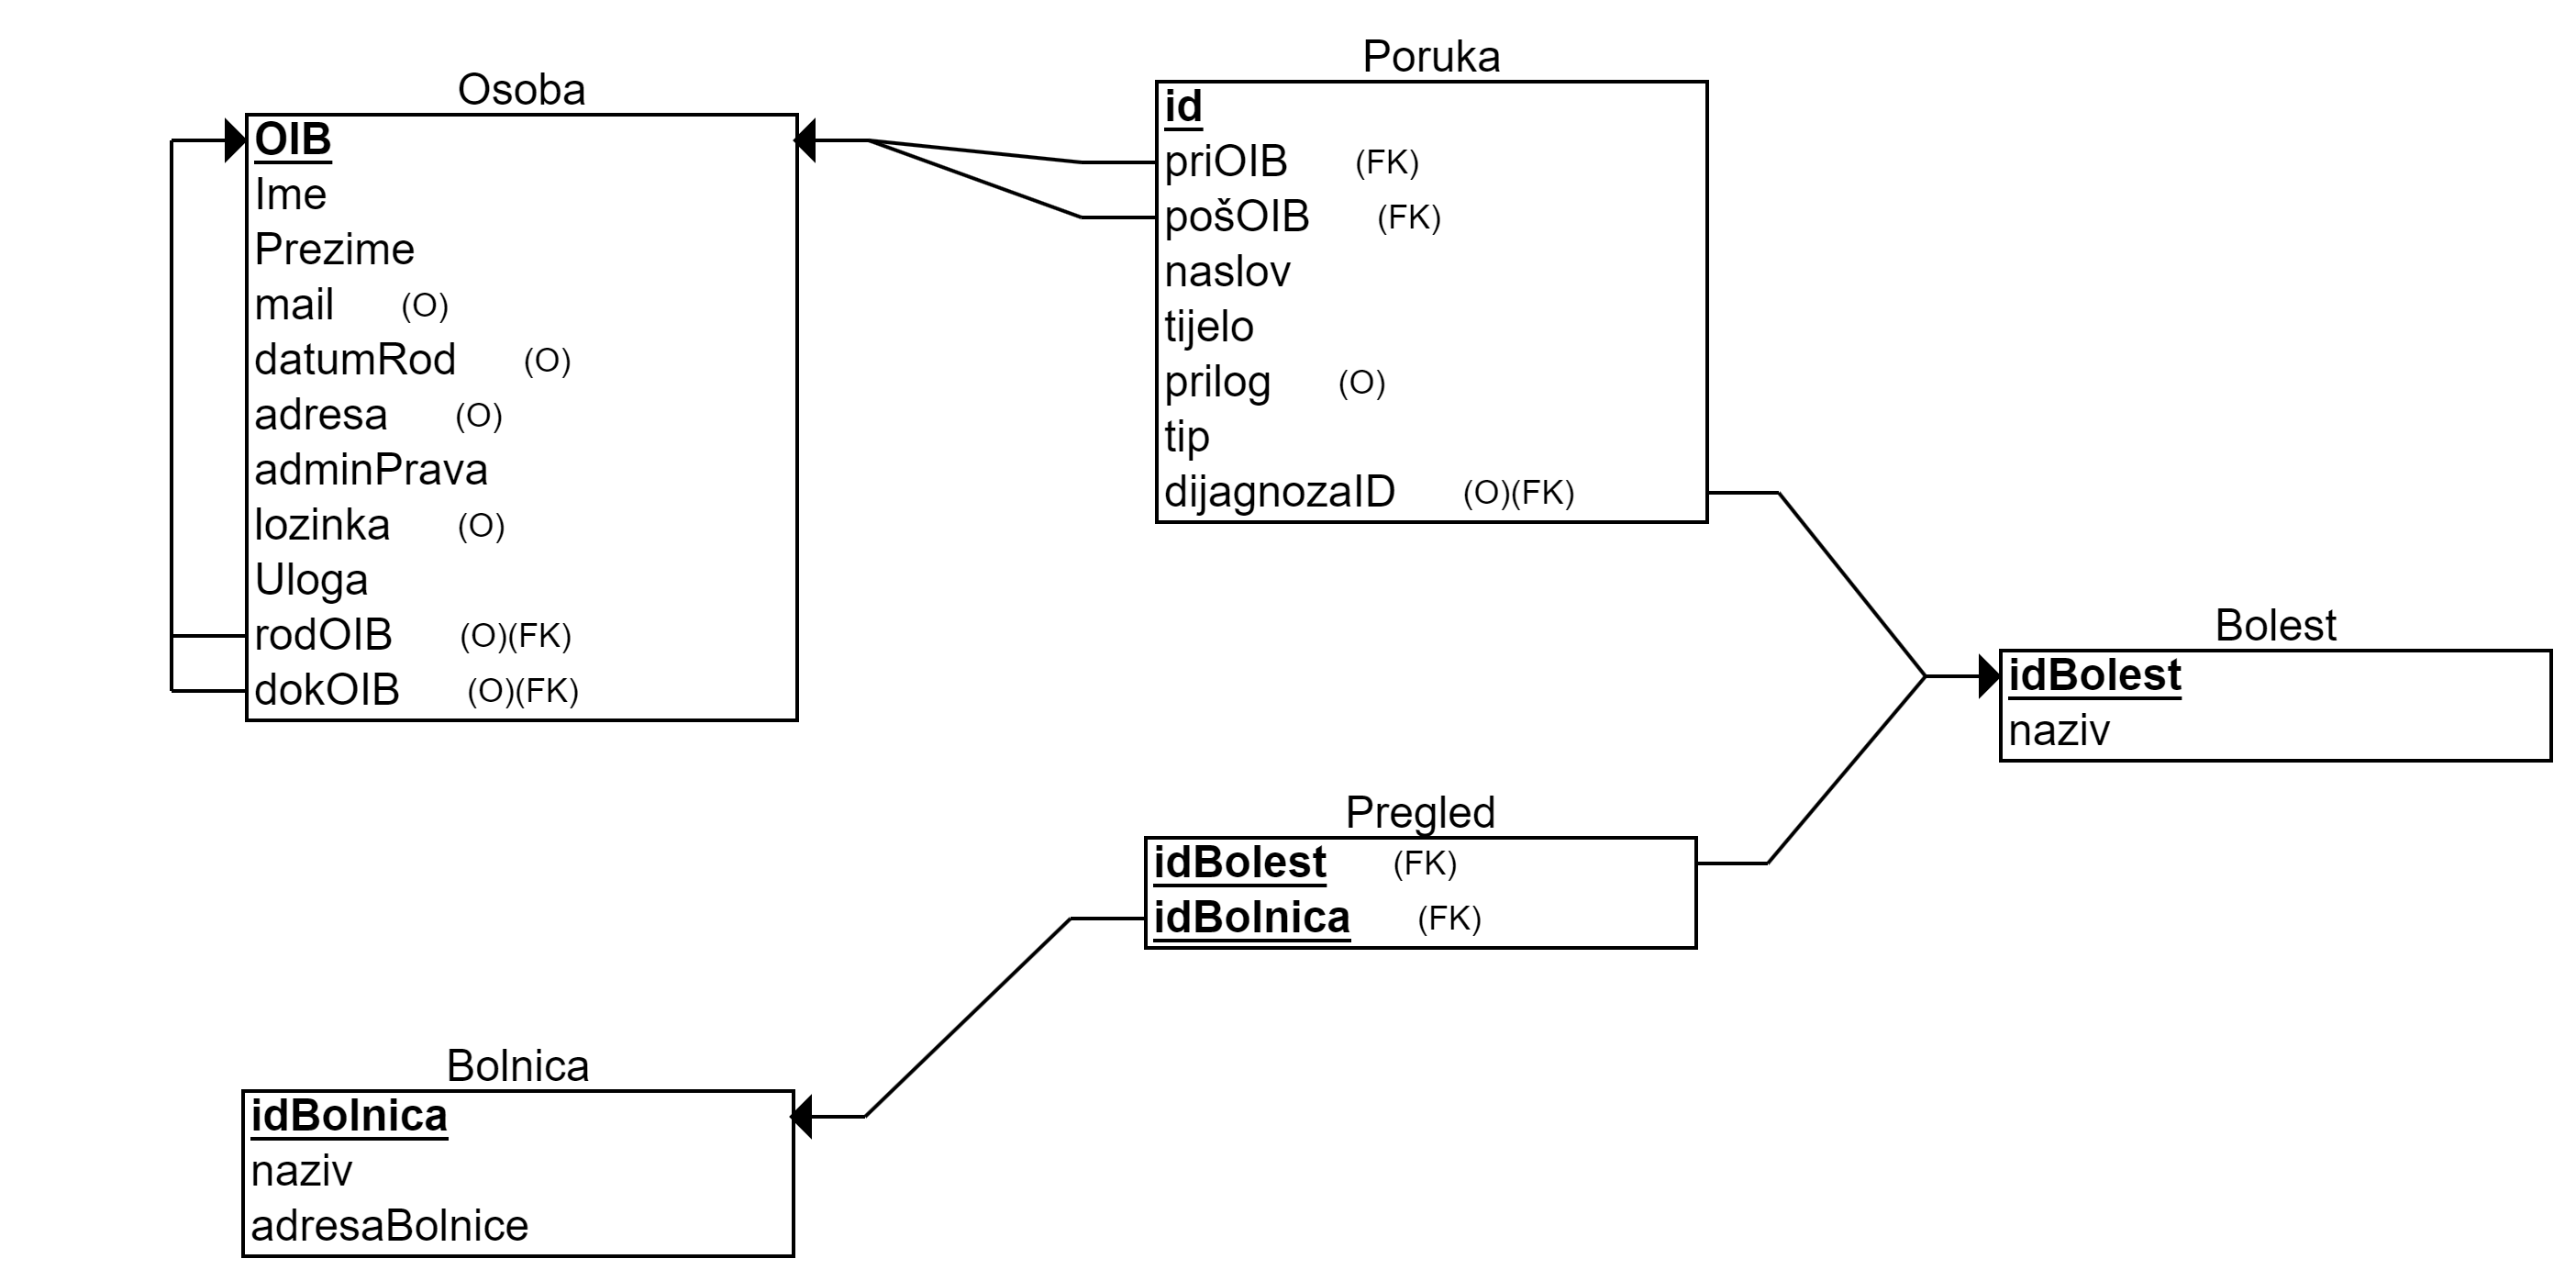
\includegraphics[width=\textwidth]{slike/dijagramBazeHigh.png} %veličina u odnosu na širinu linije
					\caption{Dijagram baze podataka}
					\label{fig:promjene10} %label mora biti drugaciji za svaku sliku
				\end{figure}
			
			\eject
			
			
		\section{Dijagram razreda}
		
			\textit{Potrebno je priložiti dijagram razreda s pripadajućim opisom. Zbog preglednosti je moguće dijagram razlomiti na više njih, ali moraju biti grupirani prema sličnim razinama apstrakcije i srodnim funkcionalnostima.}\\
			
			\textbf{\textit{dio 1. revizije}}\\
			
			\textit{Prilikom prve predaje projekta, potrebno je priložiti potpuno razrađen dijagram razreda vezan uz \textbf{generičku funkcionalnost} sustava. Ostale funkcionalnosti trebaju biti idejno razrađene u dijagramu sa sljedećim komponentama: nazivi razreda, nazivi metoda i vrste pristupa metodama (npr. javni, zaštićeni), nazivi atributa razreda, veze i odnosi između razreda.}\\
			
			\textbf{\textit{dio 2. revizije}}\\			
			
			\textit{Prilikom druge predaje projekta dijagram razreda i opisi moraju odgovarati stvarnom stanju implementacije}
			
			
			
			\eject
		
		\section{Dijagram stanja}
			
			
			\textbf{\textit{dio 2. revizije}}\\
			
			\textit{Potrebno je priložiti dijagram stanja i opisati ga. Dovoljan je jedan dijagram stanja koji prikazuje \textbf{značajan dio funkcionalnosti} sustava. Na primjer, stanja korisničkog sučelja i tijek korištenja neke ključne funkcionalnosti jesu značajan dio sustava, a registracija i prijava nisu. }
			
			
			\eject 
		
		\section{Dijagram aktivnosti}
			
			\textbf{\textit{dio 2. revizije}}\\
			
			 \textit{Potrebno je priložiti dijagram aktivnosti s pripadajućim opisom. Dijagram aktivnosti treba prikazivati značajan dio sustava.}
			
			\eject
		\section{Dijagram komponenti}
		
			\textbf{\textit{dio 2. revizije}}\\
		
			 \textit{Potrebno je priložiti dijagram komponenti s pripadajućim opisom. Dijagram komponenti treba prikazivati strukturu cijele aplikacije.}
	\chapter{Implementacija i korisničko sučelje}
		
		
		\section{Korištene tehnologije i alati}
		
			\textbf{\textit{dio 2. revizije}}
			
			 \textit{Detaljno navesti sve tehnologije i alate koji su primijenjeni pri izradi dokumentacije i aplikacije. Ukratko ih opisati, te navesti njihovo značenje i mjesto primjene. Za svaki navedeni alat i tehnologiju je potrebno \textbf{navesti internet poveznicu} gdje se mogu preuzeti ili više saznati o njima}.
			 
			 Za potrebe rada na projektu, tim je komunicirao preko aplikacija WhatsApp\footnote{https://www.whatsapp.com/} i Discord\footnote{https://discord.com/}. 
			 Za izradu UML dijagrama, korišten je alat Astah\footnote{https://astah.net/}.
			 Za upravljanje različitim verzijama datoteka korišten je sustav Git\footnote{https://git-scm.com/}.
			 Udaljeni repozitorij projekta nalazi se na platformi Github\footnote{https://github.com/}. Za izradu i testiranje baze korišten je sustav za upravljanje bazama podataka PostgreSQL\footnote{https://www.postgresql.org/}.
			 
			 Kao integrirano razvojno okruženje (IDE) korišten je Intellij IDEA\footnote{https://www.jetbrains.com/idea/}. Ovaj IDE razvio je JetBrains. Koristi se prvenstveno za razvoj softvera napisanog u Javi, Kotlinu i drugim JVM (Java Virtual Machine) jezicima. Preko pluginova nudi podršku i za mnoge druge programske jezike kao što su Python, R, Julia itd. Za potrebe rada na projektu, tim je koristio studentske licence za navedeni IDE preko kojih je moguće koristiti podršku Intellij-a za razne radne okvire (npr. Spring, React).
			 
			 Aplikacija \textit{Ozdravi} napisana je koristeći radni okvir React\footnote{https://react.dev/} za \textit{frontend} te radni okvir Spring\footnote{https://spring.io} za \textit{backend}.
			 \textit{React} je Javascript biblioteka otvorenog koda za izradu korisničkih sučelja. Održavaju ju Meta i zajednica programera i tvrtki. Ova biblioteka brza je i jednostavna za koristiti te se pomoću nje najčešće razvijaju single-page aplikacije. Velika prednost toga je što React omogućuje da se prilikom korištenja sučelja ponovno naslikaju (renderaju) samo dijelovi koji su se izmijenili. Sučelje izrađeno pomoću Reacta sastavljeno je od komponenti koje se mogu ponovno iskoristiti.
			 \textit{Spring} je besplatan radni okvir za razvoj aplikacija u Javi (i drugim jezicima). Vrlo je popularan zbog različitih modula koje nudi čime se znatno ubrzava stvaranje aplikacije. U sklopu izrade ove aplikacije korišteni su Spring Boot (razvoj aplikacije s minimalnom količinom konfiguracija), Spring Security (jednostavna konfiguracija zaštite aplikacije), Spring Data JPA (za lakšu komunikaciju s bazom podataka) i drugi. Za brzo početno podešavanje korištena je stranica Spring initializr\footnote{https://start.spring.io/}.
				
			
			\eject 
		
	
		\section{Ispitivanje programskog rješenja}
			
			\textbf{\textit{dio 2. revizije}}\\
			
			 \textit{U ovom poglavlju je potrebno opisati provedbu ispitivanja implementiranih funkcionalnosti na razini komponenti i na razini cijelog sustava s prikazom odabranih ispitnih slučajeva. Studenti trebaju ispitati temeljnu funkcionalnost i rubne uvjete.}
	
			
			\subsection{Ispitivanje komponenti}
			\textit{Potrebno je provesti ispitivanje jedinica (engl. unit testing) nad razredima koji implementiraju temeljne funkcionalnosti. Razraditi \textbf{minimalno 6 ispitnih slučajeva} u kojima će se ispitati redovni slučajevi, rubni uvjeti te izazivanje pogreške (engl. exception throwing). Poželjno je stvoriti i ispitni slučaj koji koristi funkcionalnosti koje nisu implementirane. Potrebno je priložiti izvorni kôd svih ispitnih slučajeva te prikaz rezultata izvođenja ispita u razvojnom okruženju (prolaz/pad ispita). }
			
			
			
			\subsection{Ispitivanje sustava}
			
			Testovi su izvršeni pomoću Selenium IDE ekstenzije za Google Chrome. Selenium IDE omogućava automatsko testiranje funkcionalnosti web stranica. Ovaj pristup olakšava identifikaciju grešaka i poboljšava efikasnost procesa testiranja, pružajući preciznost i brzinu u otkrivanju potencijalnih problema.\\ 
				Sam proces testiranja sastoji se od snimanja korisnikovih akcija koje se zatim spremaju kao test. Svaki test moguće je višetruko pokretat te mijenjat unesene parametre. U dokumentaciji je prikazano i opisano testiranje četiri osnovna obrasca uporabe (UC2, UC7, UC24, UC5).\\
			
			\noindent \textbf{Prvi test} provjerava proces prijave u sustav već registriranog korisnika (UC2 - Prijavi se). Tijek testiranja:\\
			Ulazi: 
			\begin{enumerate}
				\item Otvaranje web stranice u pregledniku.
				\item Pritisak na gumb „Prijava“.
				\item Pritisak polja „oib“.
				\item Unos OIB-a postojećeg korisnika.
				\item Pritisak polja „password“
				\item Unos lozinke postojećeg korisnika.
				\item Pritisak na gumb „prijava“.
			\end{enumerate}
			
			\noindent Očekivani rezultat: prikaz stranice korisničkog profila.\\
			Rezultat: očekivani rezultat je zadovoljen i aplikacija prolazi test.
			
			\begin{figure}[H]
				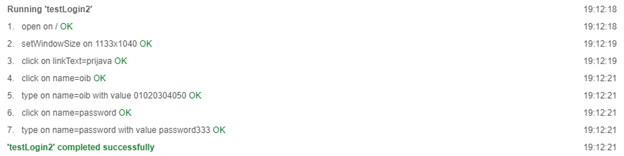
\includegraphics[width=\textwidth]{slike/prijavaUSustav.PNG} %veličina u odnosu na širinu linije
				\caption{Rezultati prvog ispitnog slučaja}
				\label{fig:prijavaTest} %label mora biti drugaciji za svaku sliku
			\end{figure}
			\eject 
		
		\noindent \textbf{Drugi test} provjerava pregled podataka o naručenom specijalističkom pregledu (UC7). \\
			Ulazi: 
		\begin{enumerate}
			\item Odabir profila.
			\item Odabir poruke s naslovom "Naručen pregled".
			\item Pritisak kursorom na kartu, pomicanje kotačića na mišu.
			\item Pritisak kursorom na jednu od označenih bolnica.
		\end{enumerate}
		
		\noindent Očekivani rezultati:\\ Prikazuje se karta sa svim bolnicama iz baze podataka koje su u blizni stanovanja pacijenta. Na karti je moguće mijenjati visinu i poziciju pogleda te otvoriti ikonu s nazivom bolnice.\\
		Rezultati: očekivani rezultat je zadovoljen i aplikacija prolazi test.
		
		\begin{figure}[H]
			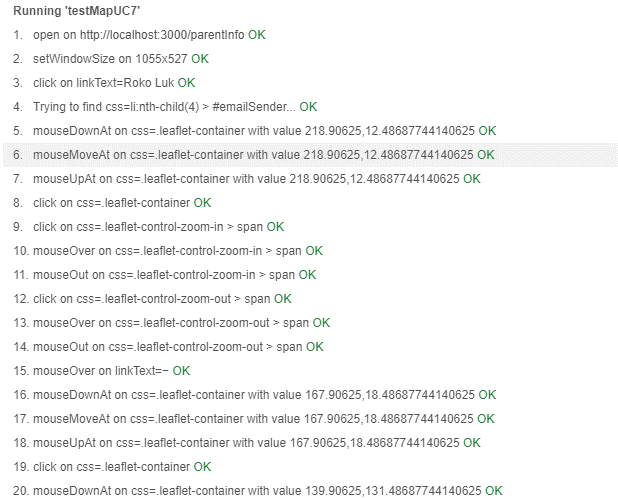
\includegraphics[width=\textwidth]{slike/pregledNaručivanja.PNG} %veličina u odnosu na širinu linije
			\caption{Rezultati drugog ispitnog slučaja}
			\label{fig:pregledKarteTest} %label mora biti drugaciji za svaku sliku
		\end{figure}
		\begin{figure}[H]
			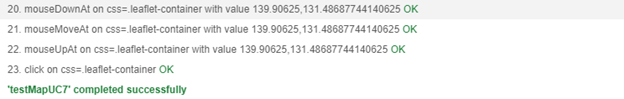
\includegraphics[width=\textwidth]{slike/pregledNaručivanja2.PNG} %veličina u odnosu na širinu linije
			\caption{Rezultati drugog ispitnog slučaja}
			\label{fig:pregledKarteTest2} %label mora biti drugaciji za svaku sliku
		\end{figure}
		
		
		\noindent \textbf{Treći test} provjerava akciju propisivanja bolovanja roditelju (UC24).\\
		Ulazi:
		\begin{enumerate}
			\item Odabir profila roditelja.
			\item Pritisak na „Nova poruka.
			\item Unos teksta poruke.
			\item Označavanje opcije „Bolovanje roditelja“.
			\item Pritisak gumba "Pošalji".
		\end{enumerate}
		Očekivani rezultati:\\Prikaz profila roditelja s novom porukom naziva "dijagnoza". Odabirom te poruke prikazuje se prikaz za čitanje poruke u kojoj vidimo sadržaj i na dnu tekst „Odobreno bolovanje“.\\
		Rezultat: Očekivani rezultat je zadovoljen. Aplikacija je prošla test.
		
		\begin{figure}[H]
			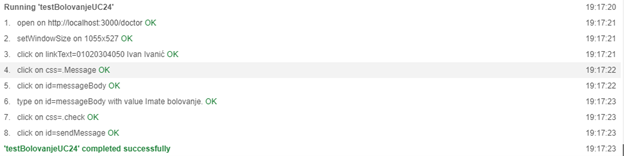
\includegraphics[width=\textwidth]{slike/propisivanjeBolovanja.PNG} %veličina u odnosu na širinu linije
			\caption{Rezultati trećeg ispitnog slučaja}
			\label{fig:propisivanjeBolovanjaTest} %label mora biti drugaciji za svaku sliku
		\end{figure}
		\eject 
		
		\noindent \textbf{Četvrti test} provjerava izmjenu osobnih podataka na stranici roditelja/djeteta (UC 5).\\
		Ulazi:
		\begin{enumerate}
			\item Odabir profila roditelja/djeteta.
			\item Pritisak ikone za izmjenu podataka.
			\item Odabir polja za izmjenu.
			\item Unos novih podataka.
			\item Pritisak na gumb "spremi.
		\end{enumerate}
		Očekivani rezultati:\\ Prikazuje se stranica korisničkog profila. Po otvaranju prozora s osobnim podatcima prikazuju se ažurirani podatci.\\
		Rezultati: Očekivani rezultat je zadovoljen. Aplikacija je prošla test.
		
		\begin{figure}[H]
			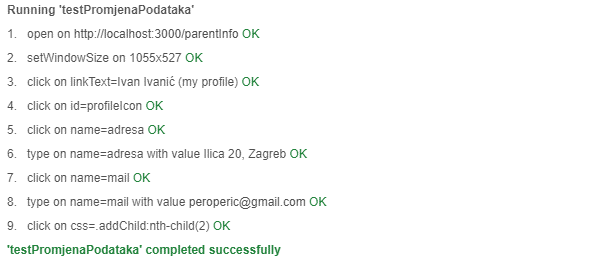
\includegraphics[width=\textwidth]{slike/promjenaPodataka.PNG} %veličina u odnosu na širinu linije
			\caption{Rezultati četvrtog ispitnog slučaja}
			\label{fig:promjenaPodatakaTest} %label mora biti drugaciji za svaku sliku
		\end{figure}
		\eject
		
		Poslijednjim testom prikazujemo kako sustav reagira ukoliko test ne prolazi. Test je proveden ponovnim pokretanjem prvog testa, no ovaj put s neispravnom lozinkom. Očekivani izlaz je neuspješna prijava korisnika te prikaz poruke o pogrešci.
		
		\begin{figure}[H]
			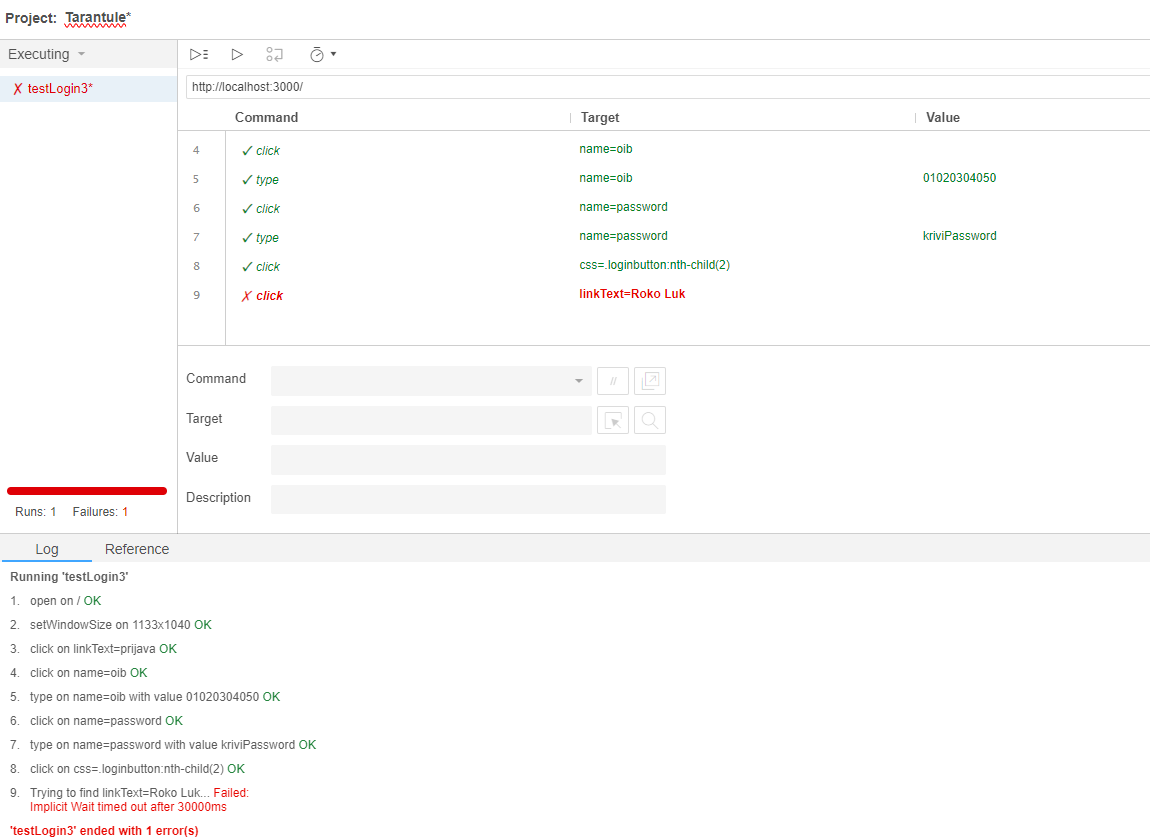
\includegraphics[width=\textwidth]{slike/neispravnaPrijava.PNG} %veličina u odnosu na širinu linije
			\caption{Rezultati i parametri petog ispitnog slučaja}
			\label{fig:neispravnaPrijavaTest} %label mora biti drugaciji za svaku sliku
		\end{figure}
		\eject
		
		\section{Dijagram razmještaja}
			
			\textbf{\textit{dio 2. revizije}}
			
			 \textit{Potrebno je umetnuti \textbf{specifikacijski} dijagram razmještaja i opisati ga. Moguće je umjesto specifikacijskog dijagrama razmještaja umetnuti dijagram razmještaja instanci, pod uvjetom da taj dijagram bolje opisuje neki važniji dio sustava.}
			 
			 Dijagram razmještaja je strukturni UML dijagram koji opisuje topologiju sustava i prikazuje odnos sklopovskih i programskih dijelova. Na slici \ref{fig:dijagramrazmjestaja} prikazan je specifikacijski dijagram razmještaja aplikacije. Na čvoru koji predstavlja korisnički uređaj nalazi se web preglednik (artefakt) korisnika. On preko HTTPS protoka komunicira s poslužiteljem. Poslužitelj pruža uslugu poslužitelja frontenda, backenda te baze podataka. Sve te usluge mogu međusobno komunicirati slanjem zahtjeva.
			 
			 \begin{figure}[H]
			 	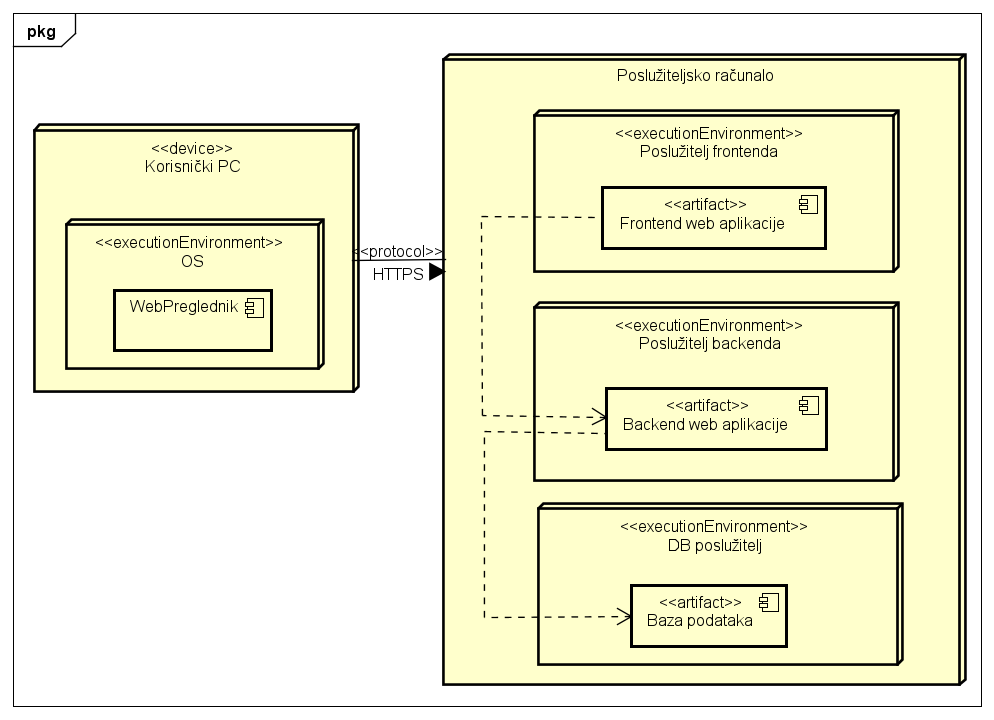
\includegraphics[width=\textwidth]{dijagrami/Dijagram razmjestaja.PNG} %veličina u odnosu na širinu linije
			 	\caption{Dijagram razmještaja}
			 	\label{fig:dijagramrazmjestaja} %label mora biti drugaciji za svaku sliku
			 \end{figure}
			
			\eject 
		
		\section{Upute za puštanje u pogon}
		
			\textbf{\textit{dio 2. revizije}}\\
		
			 \textit{U ovom poglavlju potrebno je dati upute za puštanje u pogon (engl. deployment) ostvarene aplikacije. Na primjer, za web aplikacije, opisati postupak kojim se od izvornog kôda dolazi do potpuno postavljene baze podataka i poslužitelja koji odgovara na upite korisnika. Za mobilnu aplikaciju, postupak kojim se aplikacija izgradi, te postavi na neku od trgovina. Za stolnu (engl. desktop) aplikaciju, postupak kojim se aplikacija instalira na računalo. Ukoliko mobilne i stolne aplikacije komuniciraju s poslužiteljem i/ili bazom podataka, opisati i postupak njihovog postavljanja. Pri izradi uputa preporučuje se \textbf{naglasiti korake instalacije uporabom natuknica} te koristiti što je više moguće \textbf{slike ekrana} (engl. screenshots) kako bi upute bile jasne i jednostavne za slijediti.}
			
			
			 \textit{Dovršenu aplikaciju potrebno je pokrenuti na javno dostupnom poslužitelju. Studentima se preporuča korištenje neke od sljedećih besplatnih usluga: \href{https://aws.amazon.com/}{Amazon AWS}, \href{https://azure.microsoft.com/en-us/}{Microsoft Azure} ili \href{https://www.heroku.com/}{Heroku}. Mobilne aplikacije trebaju biti objavljene na F-Droid, Google Play ili Amazon App trgovini.}
			
			
			\eject 
	\chapter{Zaključak i budući rad}
		
		 
		 Cilj rada na ovom projektu bio je napraviti aplikaciju koja omogućava roditeljima s često bolesnom djecom i liječnicima te pedijatrima lakše dogovaranje oko pregleda, slanje nalaza, slanje ispričnica te odobravanje bolovanja. Tijekom rada na projektu najveći je izazov bio što nijedan član tima nije bio upoznat s načinom izrade aplikacija koristeći Spring Boot i React. Članovi su puno vremena uložili u samo upoznavanje s tehnologijama te bi ovaj projekt bio puno lakši da su ta znanja već bila stečena. 
		 
		 Rad na projektu trajao je 11 tjedana. U prvih 5 tjedana članovi su stekli znanja o tome kako organizirati funkcionalne i ostale zahtjeve sustava te iz njih napisati obrasce uporabe. Naučili su pomoću njih izraditi sekvencijski dijagram te dijagram obrazaca uporabe. Također su se upoznali s arhitekturom mobilne aplikacije te izradom baze podataka.
		 
		 U idućih 6 tjedana članovi su uglavnom radili na implementaciji projekta. Upoznali su se sa strukturom koda u Springu te načinu funkcioniranja React stranica. Veliki je dio izazova bio i sinkronizacija backenda i frontenda jer se prilikom njihovog prvotnog spajanja uočilo puno greški. Osim toga, članovi su se upoznali i s ostatkom UML dijagrama: dijagram stanja, aktivnosti, komponenti te razmještaja.
		 
		 Sudjelovanje na projektu bilo je vrlo korisno iskustvo. Članovi su osim stečenih znanja o navedenih tehnologija imali priliku iskusiti timski rad u kojem su organizacija i međusobno pomaganje ključni za uspjeh. Ovo je također mnogim članovima bio prvi doticaj s ozbiljnijim projektom u kojem postoje strogi vremenski rokovi. Svi su članovi zadovoljni sa stečenim znanjem i iskustvom.
		
		\eject 
	\chapter*{Popis literature}
		\addcontentsline{toc}{chapter}{Popis literature}
	 	
 		\textbf{\textit{Kontinuirano osvježavanje}}
	
		\textit{Popisati sve reference i literaturu koja je pomogla pri ostvarivanju projekta.}
		
		
		\begin{enumerate}
			
			
			\item  Programsko inženjerstvo, FER ZEMRIS, \url{http://www.fer.hr/predmet/proinz}
			
			\item  I. Sommerville, "Software engineering", 8th ed, Addison Wesley, 2007.
			
			\item  T.C.Lethbridge, R.Langaniere, "Object-Oriented Software Engineering", 2nd ed. McGraw-Hill, 2005.
			
			\item  I. Marsic, Software engineering book``, Department of Electrical and Computer Engineering, Rutgers University, \url{http://www.ece.rutgers.edu/~marsic/books/SE}
			
			\item  The Unified Modeling Language, \url{https://www.uml-diagrams.org/}
			
			\item  Astah Community, \url{http://astah.net/editions/uml-new}
		\end{enumerate}
		
		 
	
	
	\begingroup
	\renewcommand*\listfigurename{Indeks slika i dijagrama}
	%\renewcommand*\listtablename{Indeks tablica}
	%\let\clearpage\relax
	\listoffigures
	%\vspace{10mm}
	%\listoftables
	\endgroup
	\addcontentsline{toc}{chapter}{Indeks slika i dijagrama}


	
	\eject 
		
	\chapter*{Dodatak: Prikaz aktivnosti grupe}
		\addcontentsline{toc}{chapter}{Dodatak: Prikaz aktivnosti grupe}
		
		\section*{Dnevnik sastajanja}
		
		\textbf{\textit{Kontinuirano osvježavanje}}\\
		
		 \textit{U ovom dijelu potrebno je redovito osvježavati dnevnik sastajanja prema predlošku.}
		
		\begin{packed_enum}
			
			\item  sastanak
			\item[] \begin{packed_item}
				\item Datum: 24. listopad 2023.
				\item Prisustvovali: T. Baće, E. Bošnjak, M. Crnolatac, B. Gabelica, A. Jerbić, J. Pavlić, V. Sivec
				\item Teme sastanka:
				\begin{packed_item}
					\item sastanak s asistenticom i demosom
					\item  razrada i analiza zahtjeva projekta
					\item  definiranje osnovnih funkcionalnosti
					\item  podjela zaduženja na projektu
				\end{packed_item}
			\end{packed_item}
			
			\item  sastanak
			\item[] \begin{packed_item}
				\item Datum: 27. listopad 2023.
				\item Prisustvovali: T. Baće, E. Bošnjak, M. Crnolatac, B. Gabelica, A. Jerbić, J. Pavlić, V. Sivec
				\item Teme sastanka:
				\begin{packed_item}
					\item  predstavljanje nacrta aplikacije
					\item  skica baze podataka
					\item  komentiranje oblikovnih obrazaca
				\end{packed_item}
			\end{packed_item}
			
			\item  sastanak
			\item[] \begin{packed_item}
				\item Datum: 7. studenoga 2023.
				\item Prisustvovali: T. Baće, E. Bošnjak, M. Crnolatac, B. Gabelica, A. Jerbić, J. Pavlić, V. Sivec
				\item Teme sastanka:
				\begin{packed_item}
					\item  sastanak s asistenticom i demosom
					\item  komentiranje i ispravak baze podataka
					\item  komentiranje dijagrama
				\end{packed_item}
			\end{packed_item}
			
			\item  sastanak
			\item[] \begin{packed_item}
				\item Datum: 15. studenoga 2023.
				\item Prisustvovali: T. Baće, E. Bošnjak, M. Crnolatac, B. Gabelica, J. Pavlić
				\item Teme sastanka:
				\begin{packed_item}
					\item  dovršavanje front end-a prve verzije aplikacije
					\item  komentiranje statusa projekta
					\item  deploy aplikacije
				\end{packed_item}
			\end{packed_item}
			%
			
		\end{packed_enum}
		
		\eject
		\section*{Tablica aktivnosti}
		
			\textbf{\textit{Kontinuirano osvježavanje}}\\
			
			 \textit{Napomena: Doprinose u aktivnostima treba navesti u satima po članovima grupe po aktivnosti.}

			\begin{longtblr}[
					label=none,
				]{
					vlines,hlines,
					width = \textwidth,
					colspec={X[7, l]X[1, c]X[1, c]X[1, c]X[1, c]X[1, c]X[1, c]X[1, c]}, 
					vline{1} = {1}{text=\clap{}},
					hline{1} = {1}{text=\clap{}},
					rowhead = 1,
				} 
			
				\SetCell[c=1]{c}{} & \SetCell[c=1]{c}{\rotatebox{90}{\textbf{Tara Baće}}} & \SetCell[c=1]{c}{\rotatebox{90}{\textbf{Eugen Bošnjak }}} &	\SetCell[c=1]{c}{\rotatebox{90}{\textbf{Mia Crnolatac }}} & \SetCell[c=1]{c}{\rotatebox{90}{\textbf{Benedicte Gabelica }}} &	\SetCell[c=1]{c}{\rotatebox{90}{\textbf{Alan Jerbić }}} & \SetCell[c=1]{c}{\rotatebox{90}{\textbf{Josip Pavlić }}} &	\SetCell[c=1]{c}{\rotatebox{90}{\textbf{Vilim Sivec }}} \\  
				Upravljanje projektom 		&  &  &  &  &  &  & \\ 
				Opis projektnog zadatka 	&  &  &  &  &  &  & \\ 
				
				Funkcionalni zahtjevi       &  &  &  &  &  &  &  \\ 
				Opis pojedinih obrazaca 	&  &  &  &  &  &  &  \\ 
				Dijagram obrazaca 			&  &  &  &  &  & 4 &  \\ 
				Sekvencijski dijagrami 		& 5 &  &  &  &  & 5 &  \\ 
				Opis ostalih zahtjeva 		& 1 &  &  &  &  &  &  \\ 

				Arhitektura i dizajn sustava	 &  &  &  &  &  &  &  \\ 
				Baza podataka				& 2 &  &  &  &  &  &   \\ 
				Dijagram razreda 			&  &  &  &  &  &  &   \\ 
				Dijagram stanja				&  &  &  &  &  &  &  \\ 
				Dijagram aktivnosti 		&  &  &  &  &  &  &  \\ 
				Dijagram komponenti			&  &  &  &  &  &  &  \\ 
				Korištene tehnologije i alati 		&  &  &  &  &  &  &  \\ 
				Ispitivanje programskog rješenja 	&  &  &  &  &  &  &  \\ 
				Dijagram razmještaja			&  &  &  &  &  &  &  \\ 
				Upute za puštanje u pogon 		&  &  &  &  &  &  &  \\  
				Dnevnik sastajanja 			& 1 &  &  &  &  &  &  \\ 
				Zaključak i budući rad 		&  &  &  &  &  &  &  \\  
				Popis literature 			&  &  &  &  &  &  &  \\  
				&  &  &  &  &  &  &  \\ \hline 
				\textit{Dodatne stavke kako ste podijelili izradu aplikacije} 			&  &  &  &  &  &  &  \\
				\textit{skica aplikacije} 				& 3 &  & 4 & 2 &  &  &  \\  
				\textit{front end} 				& 8 &  & 10 &  &  &  & 10 \\  
				\textit{izrada baze podataka} 		 			&  &  &  &  &  &  & \\  
				\textit{spajanje s bazom podataka} 							&  &  &  &  &  &  &  \\ 
				\textit{back end} 							&  & 13 &  &  &  &  &  \\ 
				\textit{deploy} 				& 3 & 4 & 3 & 3 &  & 3 &  \\  
				 							&  &  &  &  &  &  &\\ 
			\end{longtblr}
					
					
		\eject
		\section*{Dijagrami pregleda promjena}
		
		\textbf{\textit{dio 2. revizije}}\\
		
		\textit{Prenijeti dijagram pregleda promjena nad datotekama projekta. Potrebno je na kraju projekta generirane grafove s gitlaba prenijeti u ovo poglavlje dokumentacije. Dijagrami za vlastiti projekt se mogu preuzeti s gitlab.com stranice, u izborniku Repository, pritiskom na stavku Contributors.}
		
	


\end{document} %naredbe i tekst nakon ove naredbe ne ulaze u izgrađen dokument 


